\documentclass[11pt,fleqn]{article}
% \documentclass[smallextended]{svjour3}

\textheight=23.3cm 
\textwidth=16.5cm 
\topmargin=-15mm 
\oddsidemargin=0cm 

\usepackage{enumerate}
\usepackage{amsmath}
\usepackage{amssymb}
\usepackage{bbm}
\usepackage{ulem}
\usepackage{graphicx}
%This package is dated and it is giving me problems
%\usepackage{subfig}
\usepackage{wrapfig}
\usepackage{pdflscape}
\usepackage[sidewaysfigure]{rotating}
\usepackage{natbib}
%\usepackage{amsthm}
%\usepackage{setspace}
\usepackage{multirow}
\usepackage{booktabs}
\newcommand{\figfile}[2]{\IfFileExists{#1}{\includegraphics[width=#2\textwidth]{#1}}{\fbox{\parbox{#2\textwidth}{\centering\small figure not yet produced: run the model script (\texttt{\detokenize{#1}})}}}}
\newcommand{\tb}{\hspace*{3mm}}
\bibpunct{(}{)}{;}{a}{,}{,}
\parskip=3mm 
\parindent=5mm 
\baselineskip=17pt
\emergencystretch=2em

\usepackage{amsthm}
\newtheorem{assumption}{Assumption}
\newtheorem{definition}{Definition}
\newtheorem{proposition}{Proposition}
\newtheorem{corollary}{Corollary}
\newtheorem{lemma}{Lemma}
\newtheorem{theorem}{Theorem}
\renewcommand{\qedsymbol}{\textit{Q.E.D.}}

\DeclareMathOperator*{\argmax}{arg\,max}
\DeclareMathOperator*{\argmin}{arg\,min}

\usepackage{algpseudocode}
\usepackage{algorithm}

\usepackage{hyperref}
\hypersetup{
  pdftitle={De Nardi, French \& Jones (2010) - Why do the Elderly Save? The Role of Medical Expenses},    % title
  pdfauthor={Robert Kirkby},     % author
  %hyperfootnotes=false,
  %hyperindex=true,
  %hyperfigures=true,  
  colorlinks=true,                % makes links a coloured word, rather than putting coloured boxes around them
  linkcolor=black,                % makes internal links black
  citecolor=black,                % makes citations black
  urlcolor=blue,                 % color of external links
  breaklinks=true                 % allow links to be brocken across multiple lines      
}


\begin{document}


%===============================
\newcommand{\rob}[1]{{\noindent\color{blue}\bf #1}}
\newcommand{\robc}[1]{{\noindent\color{blue}\bf R: #1}}
%===============================

\title{De Nardi, French \& Jones (2010) - Why do the Elderly Save? The Role of Medical Expenses}
\author{Robert Kirkby} 
\date{\today}
\maketitle
Brief description of the replication of \cite*{DeNardiFrenchJones2010}. I make few notational changes, mainly that age is $j$ here instead of $t$ in the original. This is not intended as a full description of the model, so much as making it clear how the model is expressed in terms of the VFI Toolkit; for a full description of the model you should consult the original paper.

\paragraph{Summary of results.} The replication estimates the model by GMM: every model moment is computed exactly from the agent distribution, with no simulated panel, where DFJ2010 use the method of simulated moments. The targets are rebuilt from the RAND HRS rather than taken from DFJ2010's extract, and the moments are the cell medians themselves rather than DFJ2010's indicator moments. The data figures reproduce closely (Figures 1, 2 and A1; for the 74-year-olds of 1996 median assets are \$60,000 for everyone and \$89,000 for the survivors, against DFJ2010's \$60,000 and \$84,000). The first-stage Tables 1 and 2 check the inputs: the medical-expense process is DFJ2010's exactly, and life expectancy at 70 is within 0.3 years of theirs for women and 0.1 to 0.6 years shorter for men.

The model with exogenous medical expenses replicates. In all four columns of Table 3, risk aversion (3.5--4.1 against 3.7--3.8), the discount factor and the consumption floor (\$2,650--2,675 against \$2,650--2,665) are within one of DFJ2010's standard errors, and the health-preference parameter is $-.31$ against their $-.21$ and $-.36$; the bequest parameters do not move from DFJ2010's values, so they are inherited rather than estimated. As in the paper, no richer specification fits meaningfully better than the benchmark. Figures 5--11 reproduce the paper's conclusions: without medical expenses the top quintile runs its wealth down by 94, and a lower consumption floor raises the saving of the rich as well as the poor, almost exactly by DFJ2010's numbers. Two effects are of a different size: the mortality bias in Figure 6 is about half as large as in the data, and removing medical-expense risk while keeping the mean (Figure 10) raises the assets of the top quintiles by more than in the paper. One caveat on Table 3: its estimates are those obtained by starting the minimiser from DFJ2010's published values, and they are not the lowest point of the objective. On the median-asset moments used here, risk aversion and the consumption floor trade off along a long valley, and started from DFJ2010's appendix estimates with the floor at \$5,000 the benchmark reaches a lower objective (86.3 against 96.5) at a risk aversion of 5.9. For the same reason, although the point estimates of DFJ2010's Table A1 column 2 replicate (risk aversion 5.86 and discount factor .963, against 6.04 and .96), their test that the floor and risk aversion are separately identified does not.

The model with endogenous medical expenses replicates more loosely. At the estimates (Table A1 column 5), the discount factor and the utility floor are within one standard error of DFJ2010's, and the two curvature parameters are below theirs (1.90 and 3.09 against 2.15 and 3.19, about three and 1.4 of the replication's standard errors). As DFJ2010 report of their own estimates, the model slightly underpredicts medical expenses (Figures 12 and A4). The two counterfactuals give the paper's conclusions: without medical expenses every quintile runs its assets down (Figure 13), and halving the floor raises saving by much less than in the exogenous model (Figure 14). Figure A2 also matches: the exogenous model puts too little weight on large medical expenses, and the endogenous model is closer. Table A1 columns 3 and 4 (alternative return series) and Figure A3 are not replicated. Section \ref{sec:results} sets out the estimates, including the valley.

We conclude that the paper broadly replicates, but that two sets of parameters are poorly identified: the bequest parameters, as DFJ2010's own standard errors also show, and, on the median moments used here, risk aversion separately from the consumption floor.

\section{The model}\label{sec:model}
The model is a 33 period life-cycle model, representing ages 70 to 102 (DFJ2010's data top out at age 102 in 1996). The model is essentially a standard consumption-savings exogenous life-cycle model, with some more complicated shock processes and parameters. The model has three exogenous states, a markov and an i.i.d on medical expenses, and a further markov on health. The model has ten permanent types, representing two genders (female and male) crossed with five income quintiles.

The household problem is,
\begin{align*}
 V(a,h,\zeta,\xi)  = & \max_{c,a'} (1+\delta h) \frac{c^{1-\upsilon}}{1-\upsilon} + s_{i,j,h} \beta E [V(a',h',\zeta',\xi')|h,\zeta] + (1- s_{i,j,h}) \beta \theta \frac{(estate+k)^{1-\upsilon}}{1-\upsilon} \\
 \text{subject to } & \\
 & c+a' = a + aftertaxincome + govtransfers - m \\
 & govtransfers=max(0,cfloor+m-aftertaxincome)  \\
 & taxableincome=r*a+earnings_{i,j} \\
 &  m=exp(m\_{}coeff_{i,j,h}+sigma\_{}coeff_{i,j,h}*\psi), \quad \psi=\zeta+\xi \\
 & \zeta' = \rho \zeta + \epsilon, \, \epsilon\sim N(0,\sigma_{\zeta,\epsilon}^2) \\
 & \xi \sim N(0,\sigma_{\xi}^2) \\
 & h' \sim \pi(h'|h; i,j) \text{is a markov process} \\
 & a' \geq 0 \\
\end{align*}
where $c$ is consumption, $a$ is assets, $m_{i,j,h}$ is medical expenses. $earnings_{i,j}$ is exogenous earnings, and depends on age, gender and income quintile. $h$ is health status and follows a markov process (that differs by age, gender and income quintile).

The calculation of $aftertaxincome$ from $taxableincome$ is omitted here but is just a straightforward calculation based on seven tax brackets and associated marginal tax rates.

Note, the government lump-sum transfer $govtransfers$ is typically zero, and will only be positive is it is needed for the household to reach the consumption floor $cfloor$ (after accounting for $m$ and $aftertaxincome$). If $govtransfers>0$, then it is enforced that $c=cfloor$ and $a'=0$ (not shown in eqns above).

$estate$ is $a'$ after deducting estate taxes, $estate=max(0,(1-\tau_e)*(a'-estateexemption))$; estate taxes have a tax rate $\tau_e$ and an exemption $estateexemption$ (DFJ2010 called these $tautilde$ and $xtilde$, respectively).

Because VFI Toolkit cannot handle conditional survival probabilities that depend on the state, we have to implement $s_{i,j,h}$ in an alternative fashion. We use just $\beta$ as the discount factor. We extend $h$ to have two further values, $h=2$ is death and $h=3$ is dead (we also need to give the warm-glow of bequests with probability $s_{i,j,h}$, hence we need to distinguish the period of death, when the warm-glow of bequests is received, from 'dead' which just gives return of zero). We then set up the transitions between $h=0$ (good health) and $h=1$ (bad health) following the health transition probabilities of DFJ2010, $\pi(h'|h; i,j)$, and set transition probabilities from $h=0,1$ to $h=2$ following (one minus the) conditional survival probabilities $s_{i,j,h}$. Transitions from $h=2$ to $h=3$ occur with probability one, and $h=3$ is an absorbing state (so probability 1 of staying in it once you are there). This is slightly wasteful computationally (we will end up carrying around all the dead households), but model is easy enough to solve that it won't be an issue.

The main complication for setting up this model is that many of these parameters depend on age, permanent type (both gender and income quintile), and some even depend on health status (good or bad). This means that the number of parameters in this model is over two-thousand. This is not difficult per se (you largely just set up the parameters as age-depedent vectors, and set different ones for each permanent type, the code will handle them trivially)\footnote{Depdendence on health status is trickier, but since it is just good or bad we just create two parameters, and then in the ReturnFn etc. we juse have an if-statement on healt status that selects which of the two is relevant.} but it does take quite a lot of lines of code to write out.

The initial distribution of agents is based on the data distribution for 1996 (as this is the first year of data for the GMM estimation). Section \ref{sec:cohorts} explains how the five birth cohorts, which enter the data at different ages, are handled.

\subsection{Normalisation of $\psi$}
DFJ2010 write medical expenses as $m=\exp(m\_{}coeff_{i,j,h}+sigma\_{}coeff_{i,j,h}\,\psi)$ with $\psi=\zeta+\xi$. Two points about the inputs are worth recording, since both were got wrong in earlier versions of these codes. First, the second medical-expense regression in the replication materials predicts the \emph{variance} of log medical expenses, not the standard deviation (the documentation calls its coefficients ``the (conditional on X) variance of log medical expenditures'', and the GAUSS and C codes take the square root before use), so $sigma\_{}coeff_{i,j,h}$ is the square root of that regression's prediction. Using the variance itself as the standard deviation is harmless at age 70, where the variance is about one, but at age 95 it turns a log standard deviation of 1.7 into 3, and the implied mean medical expense $\exp(m+\sigma^2/2)$ is then overstated by a factor of about twenty. Second, $\psi$ has unit variance by construction: Table 1's estimates give $0.050/(1-0.922^2)+0.665=0.999$, and the C code fixes the AR(1) share and the white-noise share of the variance to sum to one. So no renormalisation of $\psi$ is needed; the codes carry a parameter $normalizepsi$ that makes this explicit (it equals $1.0$). An earlier formula, which used $\sigma_\varepsilon/(1-\rho)$ instead of $\sigma_\varepsilon/\sqrt{1-\rho^2}$ for the AR(1) standard deviation, gave $2.98$ and shrank the shock to a third of its size.

\subsection{Warm-glow of bequests}
DFJ2010 estimate the model from its first-order conditions, so only the derivative of the warm-glow function enters their estimation and the paper writes the function without the additive constant that the derivative loses. An earlier version of these codes used the bequest curvature as $k=215$, which made the warm-glow enormous at small estates and led households to save far too much. Table 3 of the paper reports $k$ ``in 000s'', and the replication codes (\texttt{gmmcrit25.g}) multiply it by 1,000 before use, so $k=215{,}000$ dollars. The C code that solves the model uses the warm-glow level $\theta\,(estate+k)^{1-\upsilon}/(1-\upsilon)$ directly, with no ``$-1$'' in the numerator, and that is what the return function here does too. With $k$ in dollars there is no problem.

Two further conventions from the replication codes: the interest rate is $r=1/0.98-1$ (the paper says ``2 percent''), the estate tax rate is $\tau_e=0.15$ with exemption \$600,000, and $\theta$ is not stored directly by DFJ2010's codes, which keep instead $\phi_0$, the ``marginal propensity to consume out of terminal wealth'', with $\theta=\big((R(1-\phi_0)/\phi_0)^{\upsilon}\big)/(R\beta)$ and $R=1/0.98$; this mapping reproduces the $\theta$ values in Table 3 exactly.

\subsection{Consumption floor}
The government transfer tops consumption up to the floor whenever resources net of medical expenses, $a+aftertaxincome-m$, fall below $cfloor$, and the household then saves nothing (\texttt{wealth20\_Singles.c} line 2257, \texttt{coh=max(coh\_pre\_transfer,cMin)}). An earlier version of these codes applied the floor only when resources were \emph{negative}. That is a large difference: with the correct medical-expense risk the poorest households were self-insuring against expenses they would in fact have had covered, and the bottom two quintiles held median assets of \$13,000--38,000 against data medians of \$0--3,000.

\subsection{The transitory medical-expense shock}
Until 27 September 2026 the grid handed to the toolkit for the i.i.d.\ shock $\xi$ was its probability vector rather than its grid points, so $\xi$ took values in $(0,0.3)$ instead of on $[-3.06,3.06]$ and two thirds of the variance of the medical-expense shock (Table 1 of the paper: 66.5 percent is transitory) was missing from the model. This was in the original version of these codes and was found only when the replication of the paper's Figure 3 gave mean medical expenses at age 100 of half the value implied by the estimated lognormal process. Every model-side result in this document is from after the correction; results obtained before it (recorded in the diaries under \texttt{SavedOutput}) are not comparable.

\section{GMM estimation}\label{sec:gmm}
Estimation is done in two steps.

In the first step, many exogenous processes and parameters are estimated from the data ---specifically, $earnings_{i,j}$, $s_{i,j,h}$, $\pi(h'|h; i,j)$, and everything for the process $m_{i,j,h}$--- which essentially involves running various logit and log-linear regressions. I omit this here, and just take the parameter estimates from the replication materials of DFJ2010.\footnote{These constitute some 2000+ parameter values (due to the dependence on age, gender, income quintile, and often health status.} DFJ2010 refer to these parameters estimated in the first stage as $\chi$.\footnote{Off topic, the estimations of the income quintile fixed effects are based on dividing the cross-section for each years data, not on dividing the lifetime incomes. Hence they ignore any income mobility between the quintiles and thus overstate the permanent differences in income between the quintiles.}

In the second step, the parameters $\upsilon$, $\beta$, $\delta$, $\theta$, $k$, and $cfloor$ are found by GMM estimation of the Life-Cycle Model.\footnote{$\upsilon$=CES utility fn param, $\beta$=discount factor, $\delta$=disutility of bad health, $\theta$=bequest intensity, $k$=bequest curvature (luxury good), $cfloor$=floor on consumption (from gov transfers). Note, these six parameters are all scalars.} DFJ2010 refer to these parameters estimated in the first stage as $\Delta$. The target moments for this second step to match median assets by cohort, age, and income quintile (note: not by gender).

``Our decision to use conditional medians rather than means reflects sample size considerations; in some pqv cells, changes in one or two individuals can lead to sizable changes in mean wealth. Sample size considerations also lead us to combine men and women in a single moment condition.''. Comment: \cite*{Cagetti2003} also targets the conditional median of wealth (while estimating essentially the model of \cite*{Carroll1997}, which is the same one as \cite*{GourinchasParker2002} estimated targeting mean consumption. \cite*{Cagetti2003} motivates it on the ground that because wealth is so skewed, targeting the mean wealth in a model with something like a 'mean earnings process' would be doomed to fail.

Note: DFJ2010 do not put the medians themselves into the moment conditions; their moment for each cell is the fraction of the data observations lying at or below the model's median, minus one half. The VFI Toolkit estimation commands instead use the difference between the data median and the model median. Both identify the same parameters, but the two criteria are not the same. Appendix \ref{app:medianmoments} explains the difference and how DFJ2010's version could be implemented in the toolkit.


\section{Data: rebuilding the targets from the RAND HRS}\label{sec:data}
The replication materials of DFJ2010 contain the cleaned AHEAD panel they used (the file \texttt{wlthmat13b.out}, 2,688 individuals alive in 1996) but I rebuild the targets from the public RAND HRS Longitudinal File (2022 release, V1) so that the whole chain from raw data to estimates is reproducible.\footnote{\texttt{DFJ2010\_DataWork.m} and the subcodes \texttt{DFJ2010\_ReadStata114.m} (a reader for the Stata-format RAND file that pulls only the needed columns), \texttt{DFJ2010\_HRSextract.m}, \texttt{DFJ2010\_Targets.m} and \texttt{DFJ2010\_InitialDist.m}. It runs in about two minutes on a CPU and can be run on its own or as \texttt{doPart(1)} of the main script.} The sample follows their Appendix B: the AHEAD entry cohort (RAND \texttt{HACOHORT} equal to 0 or 1; the value 3 is the HRS cohort, a trap), single in every wave from 1993 to 2006, retired (labour earnings never above \$3,000), which gives 3,316 individuals against their 3,259. Net worth is the RAND total (\texttt{HwATOTB}), top-coded at \$2 million as in their GAUSS code; permanent income is the percentile rank of the individual's average over all observed waves of social security, SSI and disability, pensions and annuities, and government transfers; bad health is self-reported fair or poor. Two conventions had to be recovered from the codes rather than the paper: every wave is deflated by the CPI of the year \emph{before} the interview, with 1997 as base (so the amounts are, in effect, in 1998 dollars), and medical expenses are the RAND out-of-pocket total divided by two (the question covers two years) plus twelve times the monthly premiums, with the raw exit-interview total in the wave of death.

The moment conditions follow \texttt{gmmcrit25.g} exactly: five cohorts defined by age in 1996 (72--76, 77--81, 82--86, 87--91, 92--102), five permanent-income quintiles, and the years 1998, 2000, 2002, 2004 and 2006; the 1996 observation is the initial condition and is never a moment; a cell-year with fewer than 10 observations is dropped together with all later years of that cell. Applied to DFJ2010's own extract these rules produce exactly their 101 moment conditions. Applied to the rebuilt panel they produce 102 (25 for each of the first three cohorts, 20 for the fourth and 7 for the fifth, whose cells are too small after 2000). The cell medians of the two extracts have a correlation of 0.96; where they differ it is mostly in the middle quintiles, because only three-quarters of individuals are assigned to the same permanent-income quintile in the two extracts. The old-age decline of the middle-quintile median that shows up in the targets is present in DFJ2010's own extract too, so it is a feature of the data and not of the rebuild.

The weighting matrix is diagonal, with the inverse of the bootstrap variance of each data median (500 resamples of individuals, \texttt{Targets.VCV\_medians}); Appendix \ref{app:medianmoments} explains why the toolkit's median-level moments need this rather than DFJ2010's indicator-moment covariance.

\section{Cohorts entering at different ages}\label{sec:cohorts}
DFJ2010 start every simulated individual from a draw of (age, sex, permanent income, health, assets) from the 1996 data, so the model population contains five cohorts that are 74, 79, 84, 89 and about 95 years old in 1996 and are then followed to 2006. The model itself is a single age-indexed problem, so the value function is solved once, but the agent distribution has to be computed separately for each cohort from its own 1996 distribution, and each target (cohort, quintile, year) is a statistic of that cohort's distribution at age $entry+(year-1996)$.

\begin{sloppypar}
VFI Toolkit handles this with two features added for this replication. The option \texttt{simoptions.jequaloneDistAge} lets \texttt{StationaryDist\_\allowbreak FHorz\_Case1} start the forward iteration at an age other than $j=1$. In the estimation commands, \texttt{estimoptions.cohortagejshifter=1} tells \texttt{EstimateLifeCycleModel\_\allowbreak PType\_\allowbreak MethodOfMoments} that \texttt{jequaloneDist} carries an extra age dimension: the slice at age $j$ is the initial distribution of the cohort that enters at $j$ (zero for ages at which no cohort enters), the target moments are given as \texttt{TargetMoments.AgeConditionalStats.\allowbreak cohortC.\allowbreak aliveqX.assets.Median} for cohort \texttt{C}, and the objective function loops over the cohorts, computing each one's distribution from its entry age and picking out the requested ages. The entry age of each cohort is the rounded mean 1996 age of its members in the initial distribution: 74, 79, 84, 89 and 94. Within a cohort the 1996 distribution is placed on the asset grid by a lottery between the two bracketing grid points (which preserves the mean), the persistent medical-expense shock $\zeta$ is drawn from its stationary distribution and $\xi$ is i.i.d., as in DFJ2010's \texttt{initdist()}. The initial distribution uses the 2,684 individuals with assets, medical expenses and health observed in 1996 (DFJ2010: 2,688), of whom 2,221 are women.
\end{sloppypar}

One difference from DFJ2010 remains: they feed each simulated individual the health and mortality path actually observed for that person in the data (\texttt{hsimtype=2}), whereas the model here draws health and death from the estimated transition probabilities. The two agree in distribution but not individual by individual.

\section{Results}\label{sec:results}
The model is solved with divide-and-conquer and the grid-interpolation layer (10 points between each pair of asset grid points), 60 exogenous states (4 health states times 15 points for $\zeta$) and 7 points for $\xi$. At DFJ2010's published benchmark parameters (Table 3 column 1) the GMM objective is 98.1, against a $\chi^2(99)$ 5 percent critical value of 123, before any estimation. The four corrections described above (the medical-expense variance, the normalisation of $\psi$, the consumption floor, and the grid of the transitory shock) were each found by looking at which cells or which figure the model missed. Part 3 of the script checks every target median against a by-hand weighted median at each run.

\paragraph{Estimation.} Table \ref{tab:table3} gives the estimates for the four specifications of DFJ2010's Table 3, each started from their published estimates and minimised with \texttt{lsqnonlin}. The weighting matrix is diagonal, the inverse of the bootstrap variances of the cell medians, and the standard errors use the standard GMM sandwich formula with the full bootstrap covariance matrix of the medians and a numerical derivative of the moments. DFJ2010 instead use the efficient weighting matrix (the inverse of the full covariance matrix of their moments), correct for simulation error, and derive the gradient of their non-differentiable indicator moments analytically. The asset grid is the one described below.

\begin{table}[htbp]
\centering
\caption{DFJ2010 Table 3: estimated structural parameters. Original (top) and replication (bottom).}\label{tab:table3}
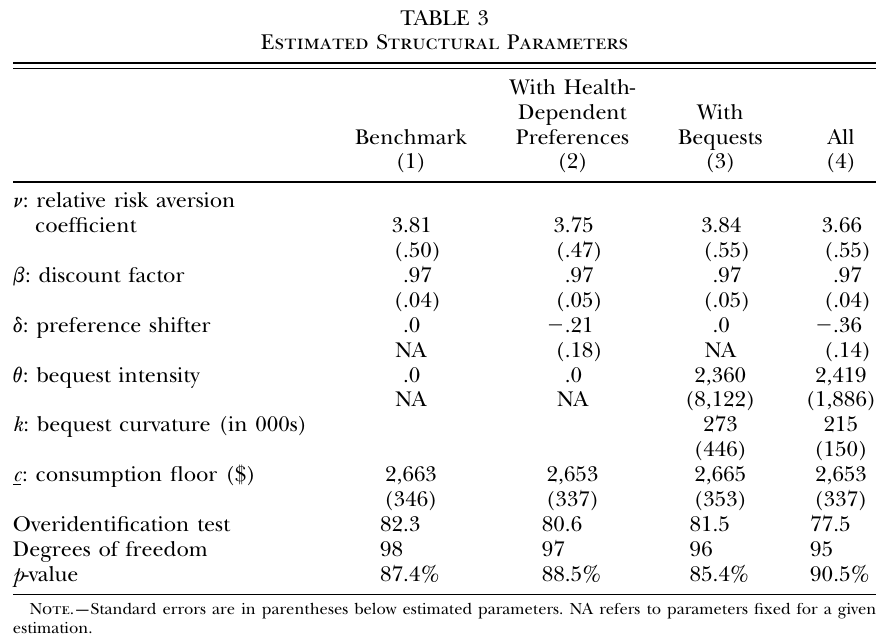
\includegraphics[width=0.7\textwidth]{./OriginalTablesFigures/DFJ2010_Table3.png}
\par\medskip
\small
\begin{tabular}{lcccc}
\toprule
 & Benchmark (1) & Health prefs (2) & Bequests (3) & All (4) \\
\midrule
$\upsilon$ & 3.72 (1.06) & 3.74 (.82) & 4.14 (.72) & 3.52 (.97) \\
$\beta$ & .967 (.119) & .972 (.100) & .934 (.081) & .970 (.112) \\
$\delta$ & 0 & $-$.31 (.15) & 0 & $-$.31 (.21) \\
$\theta$ & 0 & 0 & 2,360 (2,000) & 2,419 (1,811) \\
$k$ (000s) & & & 273 (145) & 215 (117) \\
$cfloor$ & 2,673 (768) & 2,653 (796) & 2,665 (530) & 2,653 (689) \\
objective & 96.5 [99] & 97.2 [98] & 94.4 [97] & 96.0 [96] \\
\bottomrule
\end{tabular}
\par\smallskip
\begin{minipage}{0.95\textwidth}\footnotesize
Replication on the 1001-point piecewise asset grid. Standard errors in parentheses, degrees of freedom in brackets. The replication has 102 moments (DFJ2010: 101). The $\chi^2$ 5 percent critical values are 123, 122, 121 and 120 for 99, 98, 97 and 96 degrees of freedom. Runtimes on an RTX 4000 Ada (20GB): one objective evaluation is 120 seconds; the four estimations took 174, 198, 271 and 299 minutes. Each column was started from DFJ2010's published estimates, and the estimates reported are where \texttt{lsqnonlin} stopped from there. They are not the lowest point of the objective: the benchmark objective has a long valley along which higher $\upsilon$ and a higher $cfloor$ fit about as well, and started from the Table A1 column 2 estimates instead the benchmark reaches an objective of 86.3 at $\upsilon=5.86$, $\beta=.963$, $cfloor=5{,}000$ (see the text below the table).
\end{minipage}
\end{table}

Three parameters replicate in every specification: the risk-aversion coefficient $\upsilon$ is 3.5--4.1 against their 3.7--3.8, within one of their standard errors in every column; the discount factor is .93--.97 against their .97; the consumption floor is \$2,650--2,675 against their \$2,650--2,665, remarkably close given that it comes from a different extract of the data. The overidentification statistics are 94--97 against their 78--82. Ours are higher for two reasons: the rebuilt targets differ from theirs (the extracts assign a quarter of individuals to different income quintiles), and the level moments with bootstrap variances are not the same criterion as their indicator moments (Appendix \ref{app:medianmoments}). The pattern across specifications is the same as theirs: none of the richer specifications fits meaningfully better than the benchmark, which is the paper's central point, that medical-expense risk rather than bequests or health-dependent preferences is what drives saving in old age. Figure \ref{fig:fit} shows the fit.

\paragraph{The valley in risk aversion and the consumption floor.} The estimates in Table \ref{tab:table3} are local: started from DFJ2010's published values, \texttt{lsqnonlin} stops close to them, but they are not where the objective is lowest. Re-estimating the benchmark from DFJ2010's Table A1 column 2 values instead (risk aversion 6.04, floor \$5,000) gives $\upsilon=5.86$ (1.42), $\beta=.963$ (.087), $cfloor=\$5{,}000$ (564), with an objective of 86.3 against 96.5 for column 1 of the table. Evaluating the objective on a grid of $\upsilon$ and $cfloor$ (with $\beta$ fixed at .965, where both estimates have it) shows why. There are not two separate minima but one long diagonal valley, along which a higher floor and a higher risk aversion offset each other: the objective is 98.4 at $\upsilon=3.75$ and $cfloor=\$2{,}500$, 91.8 at 4.5 and \$3,500, 88.4 at 5.25 and \$5,000, 87.1 at 6 and \$5,000, and stays at 88--90 up to $\upsilon=7.5$ with the floor at \$6,500. Off the valley it rises steeply (331.7 at $\upsilon=3$ with a floor of \$10,000, 978 at $\upsilon=7.5$ with a floor of \$1,500). The economics of the valley is that the two parameters move saving in the same direction in different parts of the distribution: a higher floor lowers the saving of the poorer quintiles, who expect to end up on it, while a higher risk aversion raises the precautionary saving of the richer ones, and on the 102 cell medians one can be traded against the other. The minimiser stops part-way down the valley from DFJ2010's start because the median moments make the objective piecewise flat (next paragraph), and in the re-estimation from the Table A1 column 2 start the floor did not move from \$5,000 at all.

The same valley decides DFJ2010's Table A1 column 2, the benchmark re-estimated with the floor fixed at \$5,000, which they use to show that the floor and risk aversion are separately identified. The point estimates replicate: $\upsilon=5.86$ (1.37) and $\beta=.963$ (.086), against their 6.04 (1.01) and .96 (.06). The test does not. For DFJ2010 the restriction raises the objective from 82.3 to 110.2, a difference of 17.9 against the $\chi^2(1)$ 5 percent critical value of 3.84, so the restriction is rejected. Here the restricted objective is 86.35, which is below column 1 of Table \ref{tab:table3} and only 0.02 above the benchmark re-estimated from the same start, so the restriction is not rejected. On the level moments used here (Appendix \ref{app:medianmoments}) risk aversion and the floor are only weakly identified separately; DFJ2010's indicator moments evidently separate them better. Table \ref{tab:table3} keeps the estimates from DFJ2010's start, as those are the comparison the table is for, and the figures in Section \ref{sec:figures} are at DFJ2010's published values in any case.

\begin{table}[htbp]
\centering
\caption{DFJ2010 appendix Table A1: estimated preference parameters. Original (top) and replication of columns 1, 2 and 5 (bottom).}\label{tab:tableA1}
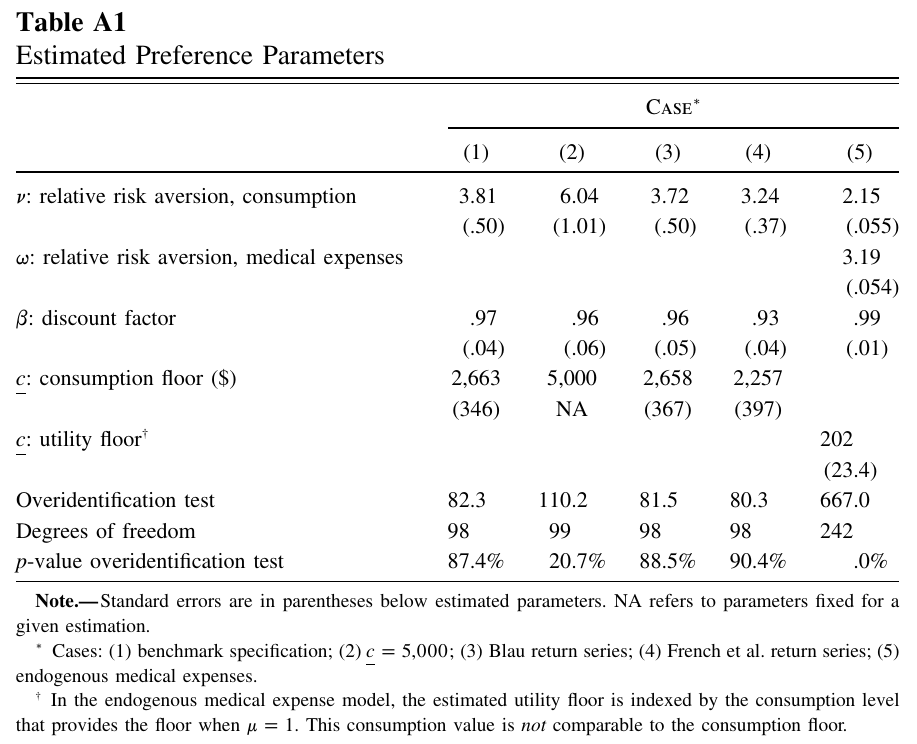
\includegraphics[width=0.7\textwidth]{./OriginalTablesFigures/DFJ2010_TableA1.png}
\par\medskip
\small
\begin{tabular}{lccc}
\toprule
 & (1) & (2) & (5) \\
\midrule
$\nu$: relative risk aversion, consumption & 3.72 (1.06) & 5.86 (1.37) & 1.90 (.082) \\
$\omega$: relative risk aversion, medical expenses & & & 3.09 (.075) \\
$\beta$: discount factor & .967 (.119) & .963 (.086) & .995 (.011) \\
$cfloor$: consumption floor (\$) & 2,673 (768) & 5,000 NA & \\
$eMin$: utility floor & & & 263 (64) \\
objective & 96.5 [99] & 86.3 [100] & 552.5 [248] \\
\bottomrule
\end{tabular}
\par\smallskip
\begin{minipage}{0.95\textwidth}\footnotesize
Standard errors in parentheses, degrees of freedom in brackets; NA: fixed. Column 1 is the benchmark, column 1 of Table \ref{tab:table3}; column 2 the benchmark with the floor fixed at \$5,000 (part 12 of the script); column 5 the model with endogenous medical expenses, estimated with the autocorrelations in DFJ2010's definition (part 8; Table \ref{tab:endog} has both definitions and the objective by block). Columns 3 and 4 (the Blau and French et al.\ realized return series) are not replicated. The column 5 objective is not on the same criterion as DFJ2010's (Table \ref{tab:endog}).
\end{minipage}
\end{table}

\begin{figure}[htbp]
\centering
\caption{DFJ2010 Figure 5: Original (top) and replication (bottom). Median assets by cohort and permanent-income quintile, data (solid) and model (dashed), at the benchmark parameters (DFJ2010 Table 3 column 1), for the cohorts aged 74 and 84 in 1996, 1996--2006. In 1996 the model's distribution is the data's, so the two lines start together; the estimation targets 1998--2006 for all five cohorts.}\label{fig:fit}
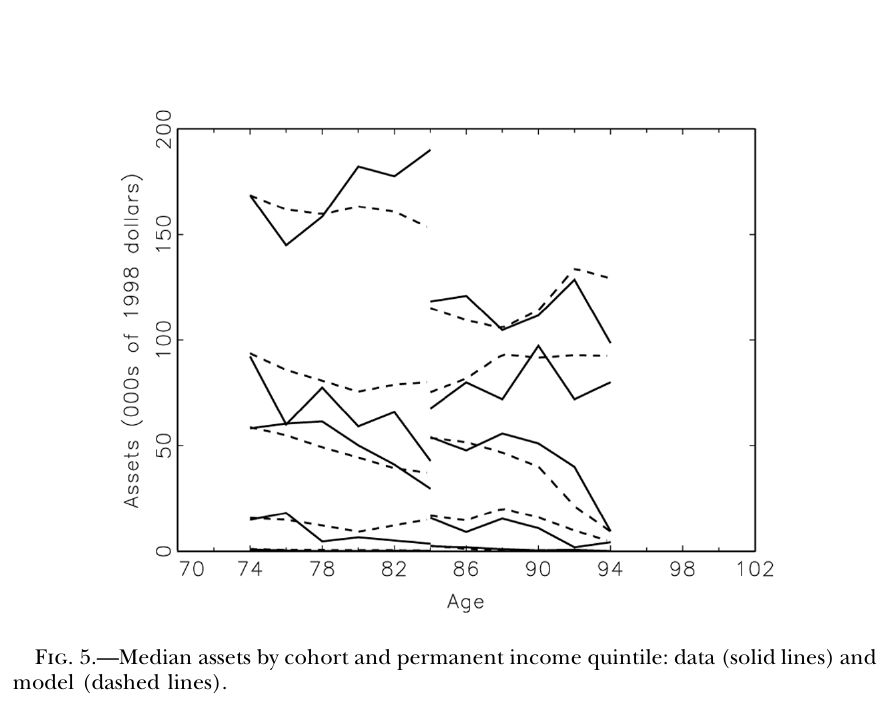
\includegraphics[width=0.55\textwidth]{./OriginalTablesFigures/DFJ2010_Figure5.png} \\
\includegraphics[width=0.75\textwidth]{../SavedOutput/Graphs/DFJ2010_Fig5_fit.png}
\end{figure}

\paragraph{The asset grid and what is identified.}
The target moments are medians, and a median sits on a grid point of the agent distribution (the distribution lives on the asset grid even though the policy is interpolated between grid points). The objective is therefore flat in a parameter until the model's median in some cell crosses a grid point, and a derivative-based minimiser sees steps of the grid spacing rather than a slope. This showed up in two ways on the cubic 501-point grid on $[0,2\text{m}]$ that the codes used originally. First, the toolkit's standard errors were absurdly small (.011 for $\upsilon$, .003 for $\beta$, \$9 for $cfloor$) because at its default finite-difference step 94--97 percent of the moments had exactly zero derivative; at the largest step (\texttt{estimoptions.eedefault=4}, about one percent of the parameter) the derivatives are meaningful and the standard errors are of the size of DFJ2010's. Second, the bequest parameters $\theta$ and $k$ did not move at all: $k$ changed by \$10 in 90 evaluations, and 88 percent of the moments had zero derivative with respect to it even at the largest step.

All 102 target medians lie between \$0 and \$280,000, but that grid put 235 of its 501 points above \$300,000 and had steps of \$1,600--3,400 in the \$100,000--300,000 range where the top quintile lives. The grid now used (\texttt{DFJ2010\_AssetGrid.m}) is piecewise: 801 points on $[0,300\text{k}]$ with quadratic spacing (steps of \$140 at \$10,000, \$430 at \$100,000, \$750 at \$300,000) and 200 points on $(300\text{k},2\text{m}]$, which only the value function uses. Two things remain even on this grid, and they are the two caveats of the replication.

The bequest parameters $\theta$ and $k$ do not move. In columns 3 and 4 the minimiser tries values a few percent away and returns to within \$30 of the starting $k$, and 85--91 percent of the moments have zero derivative in $\theta$ and $k$ at the largest step. So $\theta$ and $k$ in the table are DFJ2010's values inherited, not estimates. Part of this is the grid, but part is genuine: the bequest parameters move the cell medians very little, which is also what DFJ2010's own standard errors on them (8,122 and 446,000 in column 3) say. Estimating them properly would need a smoother criterion, either kernel-smoothed model medians or DFJ2010's own indicator moments via \texttt{estimoptions.CustomModelStats} (Appendix \ref{app:medianmoments}), or a derivative-free minimiser.

The health-preference parameter $\delta$ replicates: $-.31$ (.15) in column 2 and $-.31$ (.21) in column 4, against DFJ2010's $-.21$ (.18) and $-.36$ (.14). It is identified by a few top-quintile and middle-quintile cells, where the weighting of the female and male types within a quintile matters most; 83--90 percent of the moments have zero derivative in $\delta$ at the largest step, and it buys at most a point or two of the objective.

\section{The paper's figures}\label{sec:figures}
This section pairs each of DFJ2010's Figures 1--4 and 6--11 with its replication, the original above the replication; the captions also quote the numbers DFJ2010 report in the text. Figure \ref{fig:fit} above is their Figure 5. Figures 3 and 4 (average medical expenses and income by quintile, simulated for the cohort aged 74 in 1996 from the first-stage profiles) are produced by part 5 of the script from the same no-attrition distribution as the counterfactuals; the first-stage profiles themselves are taken from DFJ2010's replication materials and are not re-estimated. Figures 12, 13, 14 and A4 are in Section \ref{sec:endog}, with the model with endogenous medical expenses. Of the appendix figures, A1 is with the data (Figure \ref{fig:dfjA1}) and A2 in Section \ref{sec:endog} (Figure \ref{fig:dfjA2}); DFJ2010's first-stage Tables 1 and 2 are with the first-stage profiles (Tables \ref{tab:table1} and \ref{tab:table2}).

\subsection{Data}
\begin{figure}[htbp]
\centering
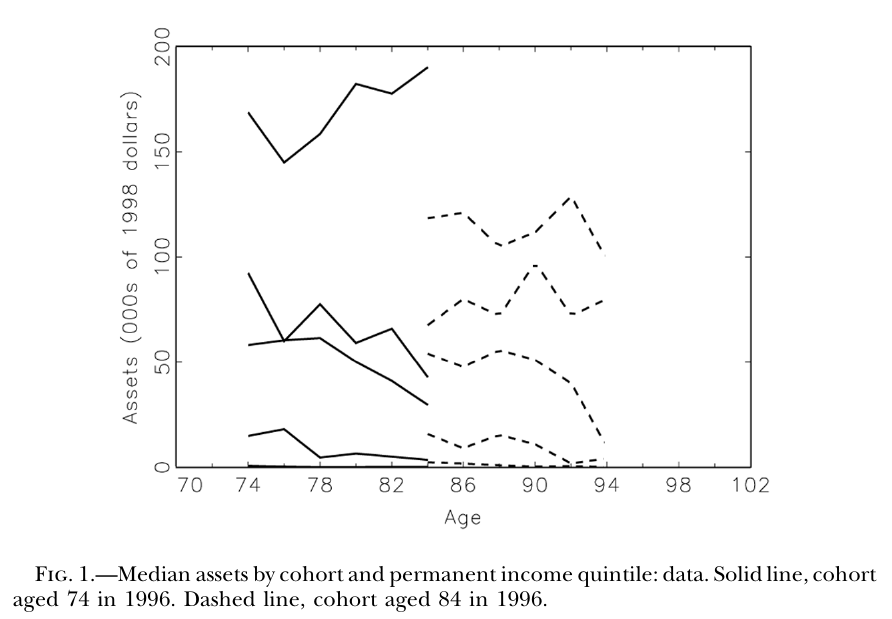
\includegraphics[width=0.6\textwidth]{./OriginalTablesFigures/DFJ2010_Figure1.png} \\
\includegraphics[width=0.7\textwidth]{../SavedOutput/Graphs/DFJ2010_DataWork_Figure1.png}
\caption{DFJ2010 Figure 1: Original (top) and replication (bottom). Median assets by cohort and permanent-income quintile in the data, for the cohorts aged 74 (solid) and 84 (dashed) in 1996, HRS rebuild. As in the paper, the top quintile of the 74-year-olds holds its assets (\$166,000 in 1996, \$212,000 in 2006 here) while the bottom two quintiles have essentially nothing throughout.}\label{fig:dfj1}
\end{figure}

\begin{figure}[htbp]
\centering
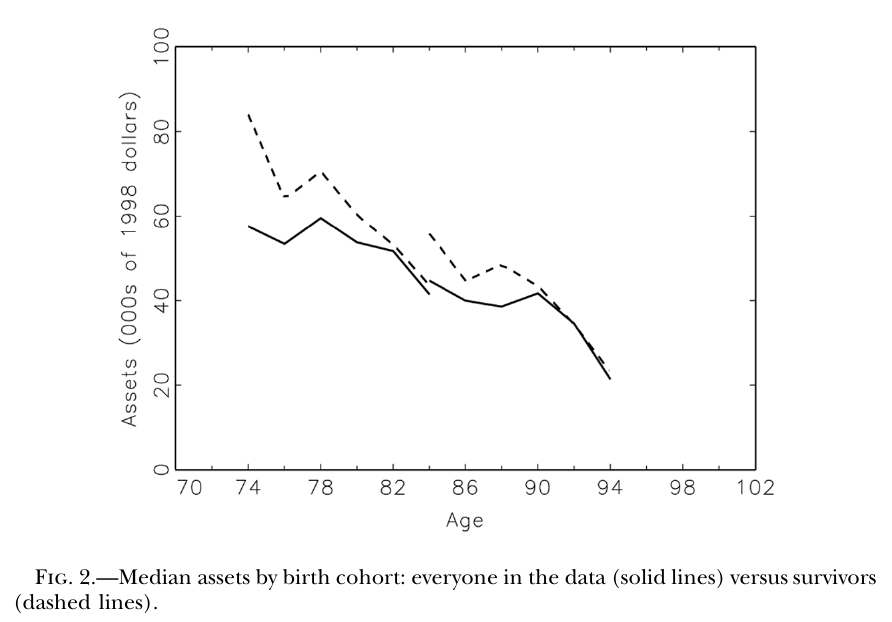
\includegraphics[width=0.6\textwidth]{./OriginalTablesFigures/DFJ2010_Figure2.png} \\
\includegraphics[width=0.7\textwidth]{../SavedOutput/Graphs/DFJ2010_DataWork_Figure2.png}
\caption{DFJ2010 Figure 2: Original (top) and replication (bottom). Median assets by birth cohort, all quintiles pooled, everyone alive at each date (solid, the unbalanced panel) against the survivors to 2006 (dashed, the balanced panel). DFJ2010 report for the 74-year-olds of 1996: median assets \$60,000 for everyone and \$84,000 for the survivors, the latter falling to \$44,000 by 2006, so the balanced panel shows a \$40,000 decline against \$16,000 for the unbalanced one. The rebuild gives \$60,000, \$89,000 and \$42,000.}\label{fig:dfj2}
\end{figure}

\begin{figure}[htbp]
\centering
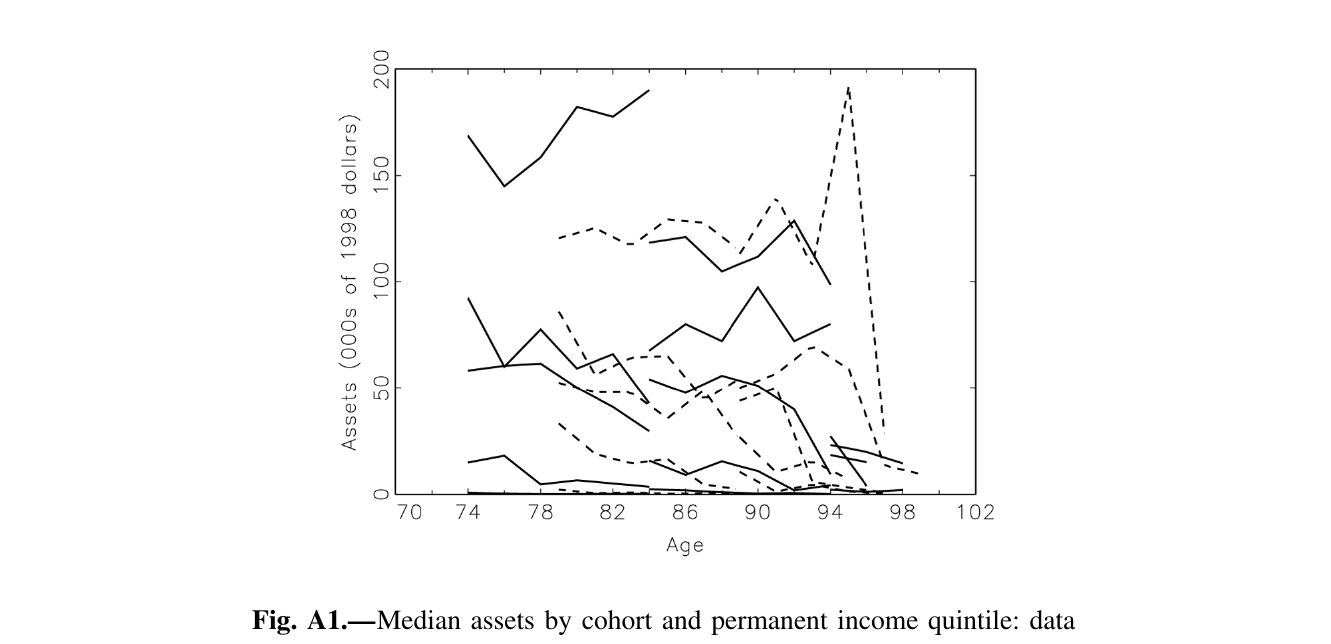
\includegraphics[width=0.75\textwidth]{./OriginalTablesFigures/DFJ2010_FigureA1.png} \\
\figfile{../SavedOutput/Graphs/DFJ2010_FigA1_data.png}{0.7}
\caption{DFJ2010 appendix Figure A1: Original (top) and replication (bottom). Median assets by cohort and permanent-income quintile in the data, HRS rebuild, 1998--2006: the 102 cells the GMM estimation targets, each line one cohort. Part 11 of the script draws it from the targets.}\label{fig:dfjA1}
\end{figure}

\subsection{First-stage profiles}
DFJ2010 draw Figures 3 and 4 by simulating medical expenses and income for the cohort aged 74 in 1996 from the estimated first-stage profiles, ``for a balanced sample of people'' (no attrition), so they are functions of the first-stage parameters, the 1996 distribution and the health dynamics only, not of the preference parameters. Part 5 of the script computes the same means from the baseline no-attrition distribution.

Tables \ref{tab:table1} and \ref{tab:table2} are DFJ2010's first-stage tables. Part 11 of the script writes Table \ref{tab:table1} directly from the parameter values the model uses, and computes Table \ref{tab:table2} from the model's health and survival transitions, so both check the inputs rather than re-estimate them. The exogenous model's medical-expense shock process is DFJ2010's Table 1 exactly. The endogenous model uses its own process, from DFJ2010's replication files, which their Table 1 does not report: less persistent (0.849) and with a larger persistent share of the variance (0.49 against 0.33). Life expectancy at 70 is the expected number of further years alive under the transitions, plus half a year for the year of death. For women it is within 0.3 years of DFJ2010's in every cell, and for men 0.1 to 0.6 years shorter. The aggregates weight the cells by the sex and health composition of the 1996 sample at all ages, since DFJ2010 do not say which ages their composition uses; for men as a group that gives 8.9 years against their 9.7, a larger gap than in any of the cells, so their composition puts more weight on healthy and richer men.

\begin{table}[htbp]
\centering
\caption{DFJ2010 Table 1: persistence and variance of innovations to medical expenses (variances as fractions of the total cross-sectional variance). Original (top) and replication (bottom).}\label{tab:table1}
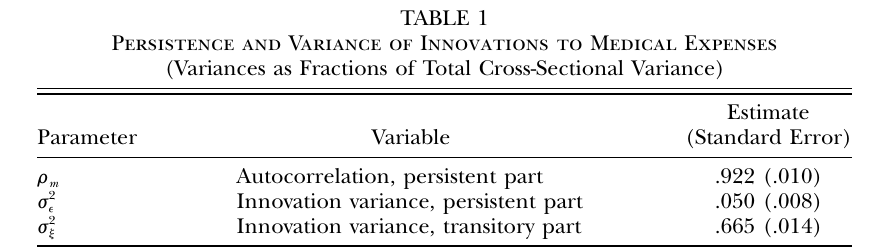
\includegraphics[width=0.7\textwidth]{./OriginalTablesFigures/DFJ2010_Table1.png}
\par\medskip
\small
\setlength{\tabcolsep}{4pt}
\input{../SavedOutput/LatexInputs/DFJ2010_Table1.tex}
\par\smallskip
\begin{minipage}{0.9\textwidth}\footnotesize
The replication columns are the values in the replication's parameters: the exogenous model's from DFJ2010's first stage, the endogenous model's from DFJ2010's replication files (\texttt{mxvec} in \texttt{singlsav51\_wave8.gau}).
\end{minipage}
\end{table}

\begin{table}[htbp]
\centering
\caption{DFJ2010 Table 2: life expectancy in years at age 70, by permanent-income quintile, sex and health at 70. Original (top) and replication from the model's transitions (bottom).}\label{tab:table2}
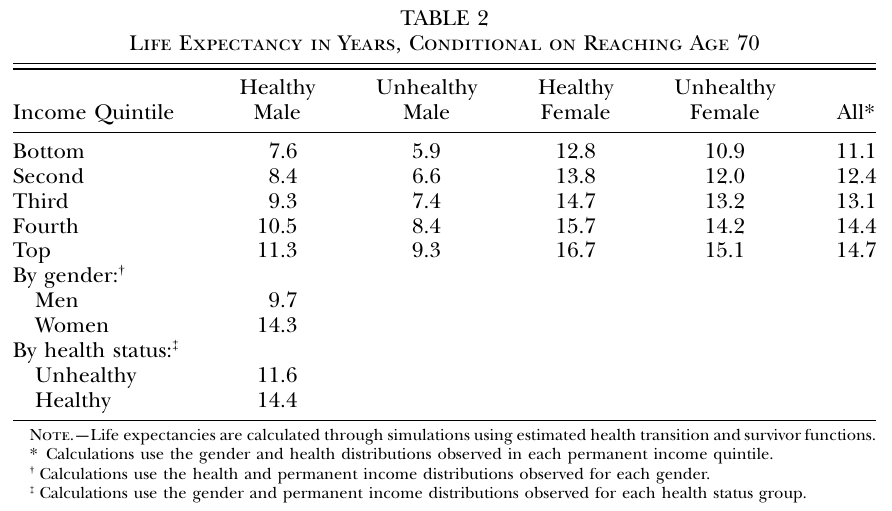
\includegraphics[width=0.7\textwidth]{./OriginalTablesFigures/DFJ2010_Table2.png}
\par\medskip
\small
\input{../SavedOutput/LatexInputs/DFJ2010_Table2.tex}
\par\smallskip
\begin{minipage}{0.9\textwidth}\footnotesize
Expected further years alive plus half a year for the year of death. All: the cells of the quintile weighted by the 1996 sample's sex and health composition within it; Men and Women, and Unhealthy and Healthy, weighted the same way within each group.
\end{minipage}
\end{table}
\begin{figure}[htbp]
\centering
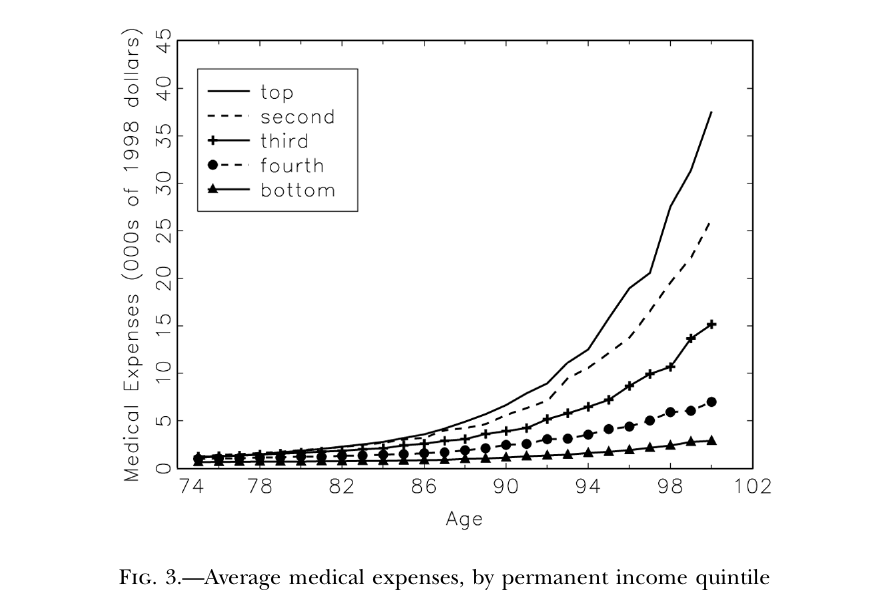
\includegraphics[width=0.6\textwidth]{./OriginalTablesFigures/DFJ2010_Figure3.png} \\
\figfile{../SavedOutput/Graphs/DFJ2010_Fig3_medex.png}{0.7}
\caption{DFJ2010 Figure 3: Original (top) and replication (bottom). Average out-of-pocket medical expenses by permanent-income quintile, cohort aged 74 in 1996 followed with no attrition. DFJ2010: ``less than \$1,000 a year at age 75'' varying little with income, rising by 100 to \$2,900 in the bottom quintile and ``almost \$38,000'' at the top. Here: \$700--1,300 at 74, and at 100 \$3,500 in the bottom quintile and \$49,000 in the top. (The model's transitory-shock bug was found through this figure: with it, the top quintile at 100 was \$19,000.)}\label{fig:dfj3}
\end{figure}
\begin{figure}[htbp]
\centering
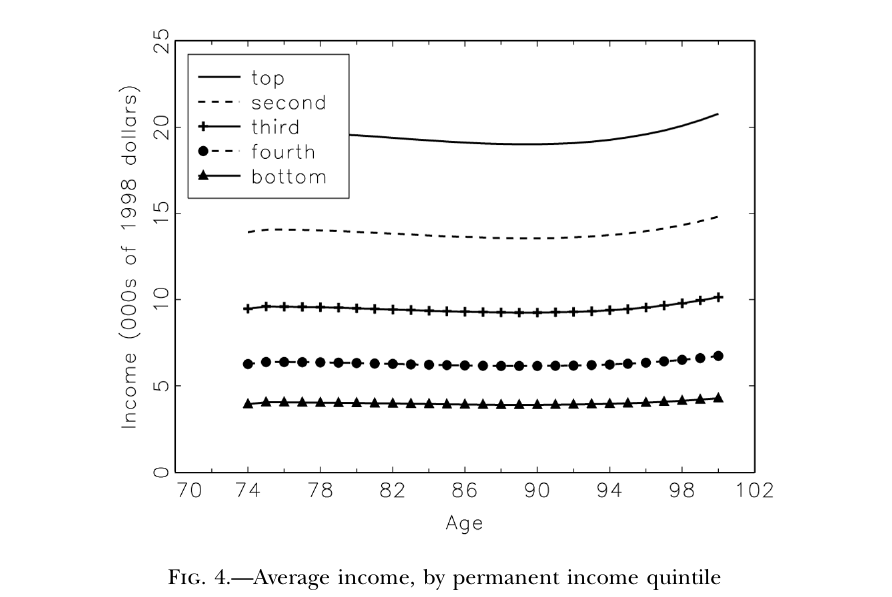
\includegraphics[width=0.6\textwidth]{./OriginalTablesFigures/DFJ2010_Figure4.png} \\
\figfile{../SavedOutput/Graphs/DFJ2010_Fig4_income.png}{0.7}
\caption{DFJ2010 Figure 4: Original (top) and replication (bottom). Average non-asset income by permanent-income quintile, same cohort. DFJ2010: ``for those in the top permanent income quintile, annual income averages \$20,000 per year''. Here the top quintile averages \$19,400 at 74, \$18,700 at 90 and \$20,400 at 100; the bottom quintile \$4,000.}\label{fig:dfj4}
\end{figure}

\subsection{Model}
Figures \ref{fig:dfj6}--\ref{fig:dfj8} are computed at the benchmark parameters (Table 3 column 1) from the cohort distributions that part 3 of the script builds for the estimation. The survivors' profiles in Figure \ref{fig:dfj6} come from reweighting each cohort's distribution at age $j$ by the probability, given health at $j$, of still being alive in 2006, which the health-and-survival chain gives directly since it does not depend on assets. The model's assets before death in Figure \ref{fig:dfj8} are the assets held by those in the death state, that is, the assets carried into the period in which the person dies, pooled over the five cohorts and the years 1997--2006; in the data they are the decedents' assets at the last interview before death (1,861 people; the paper's footnote 5 explains why they use this rather than reported estates).

\begin{figure}[htbp]
\centering
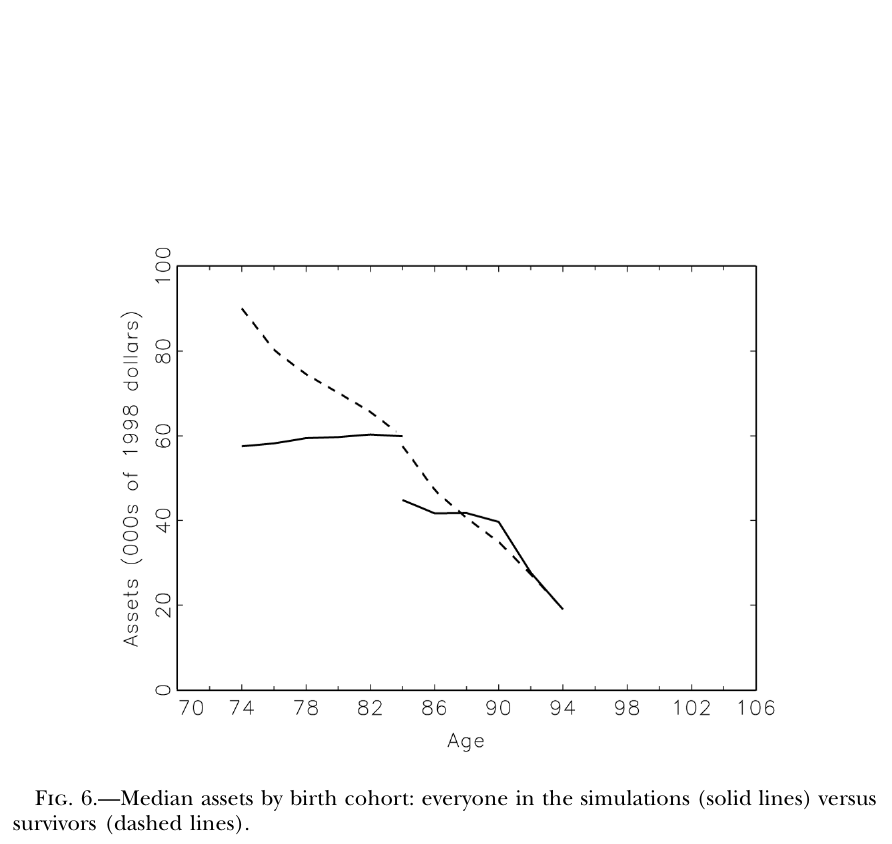
\includegraphics[width=0.55\textwidth]{./OriginalTablesFigures/DFJ2010_Figure6.png} \\
\includegraphics[width=0.7\textwidth]{../SavedOutput/Graphs/DFJ2010_Fig6_survivors.png}
\caption{DFJ2010 Figure 6: Original (top) and replication (bottom). Median assets by birth cohort in the model, everyone alive (solid) versus survivors to 2006 (dashed). The paper's point is that ``restricting the profiles to long-term survivors reveals much more asset decumulation'' in the model as in the data. Here, for the cohort entering at 74: everyone \$60,000 at entry, survivors \$70,000 at entry falling to \$50,000 in 2006; the data (Figure \ref{fig:dfj2}) have \$60,000, \$89,000 and \$42,000. The model reproduces the mortality bias but at about half its size in the data: those who die in the model hold less than the survivors mainly because they are in bad health and poorer, whereas in the data the gap at entry is larger.}\label{fig:dfj6}
\end{figure}

\begin{figure}[htbp]
\centering
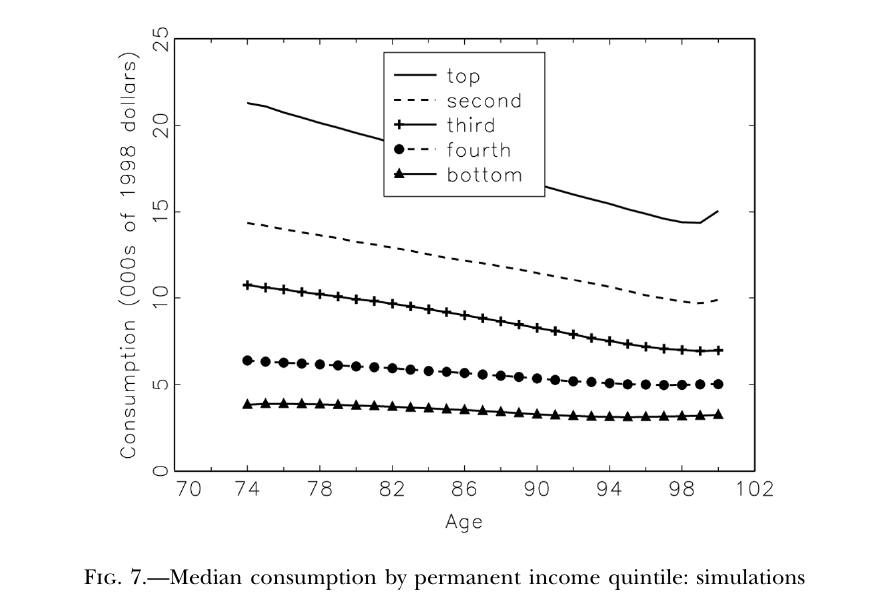
\includegraphics[width=0.6\textwidth]{./OriginalTablesFigures/DFJ2010_Figure7.png} \\
\includegraphics[width=0.7\textwidth]{../SavedOutput/Graphs/DFJ2010_Fig7_consumption.png}
\caption{DFJ2010 Figure 7: Original (top) and replication (bottom). Median consumption by permanent-income quintile in the model, the cohort aged 74 in 1996 followed to age 100. DFJ2010: ``except for the last two years of life, consumption falls with age''. The same here: median consumption falls with age in every quintile, the top quintile's turning up in the last two years, while the bottom quintile sits at the floor throughout.}\label{fig:dfj7}
\end{figure}

\begin{figure}[htbp]
\centering
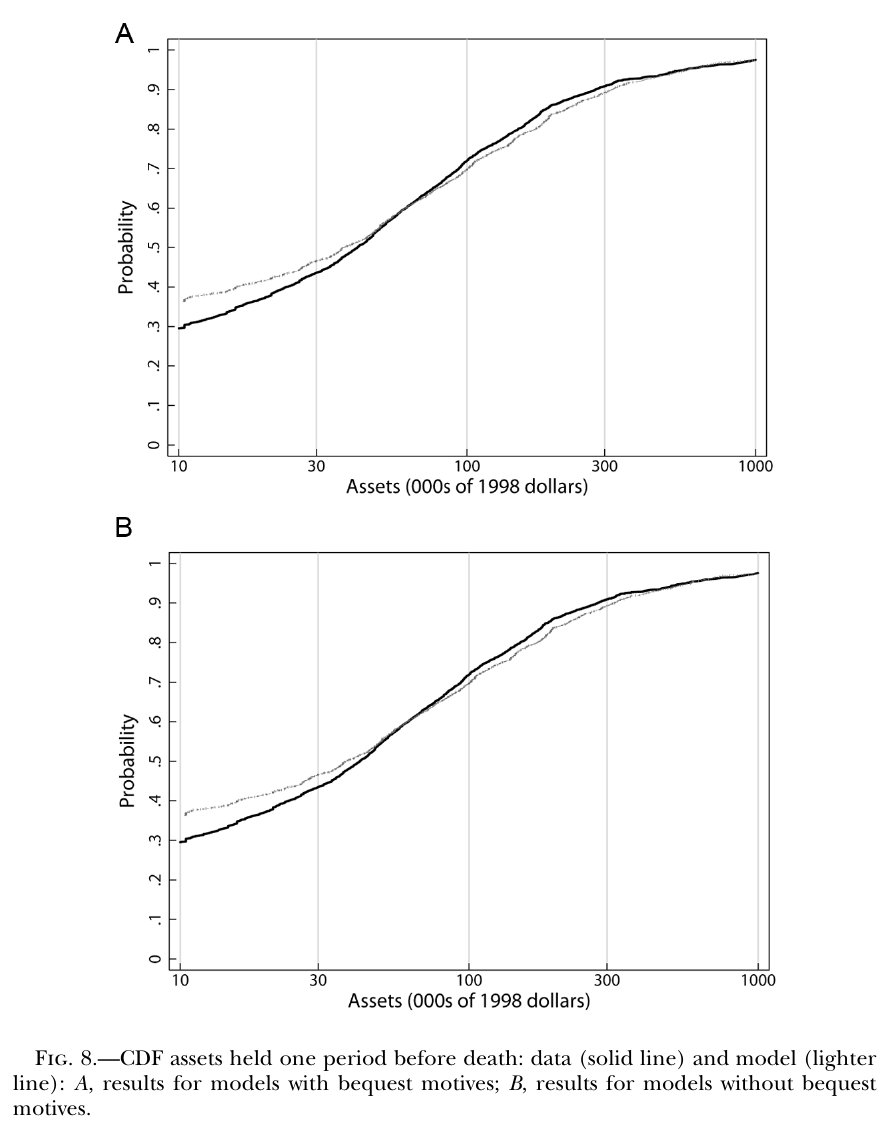
\includegraphics[width=0.42\textwidth]{./OriginalTablesFigures/DFJ2010_Figure8.png} \\
\figfile{../SavedOutput/Graphs/DFJ2010_Fig8_AB_assetsbeforedeath.png}{0.8}
\caption{DFJ2010 Figure 8: Original (top) and replication (bottom). CDF of assets held one period before death, data (solid) and model (dashed); A, the model with bequest motives (Table 3 column 3, the one DFJ2010 focus on), B, the benchmark without them (column 1), both at DFJ2010's published values. In the data (HRS rebuild) the quartiles are \$0, \$26,000 and \$108,000, with 21 percent of decedents holding nothing; in panel B the model's are \$1,000, \$29,000 and \$106,000, with 16 percent at the zero grid point, and in panel A \$1,000, \$29,000 and \$105,000, again with 16 percent at zero: the bequest motive barely changes the distribution, DFJ2010's conclusion from the same comparison. This is not a targeted moment, and DFJ2010 use it as their check that the benchmark model ``fits the data closely ... in terms of the distribution of bequests that it generates''; the two CDFs here are within a few percentage points of each other everywhere above \$20,000.}\label{fig:dfj8}
\end{figure}

\subsection{Counterfactuals}
DFJ2010 Section VIII fixes the benchmark parameters, changes one feature of the model at a time, and shows median assets by quintile for the cohort aged 74 in 1996, followed to age 100 with no attrition: ``people will face the same risks and have the same expectations as before, but in their realized lives, they do not die''. Part 5 of the script does exactly this: the policy is solved with mortality risk, and the distribution is then iterated with the health transitions conditional on survival, which the toolkit allows because the stationary-distribution command takes its own transition matrix. Three experiments: all out-of-pocket medical expenses set to zero (Figure \ref{fig:dfj9}); the medical-expense shocks $\zeta$ and $\xi$ removed while the mean expense conditional on age, type and health is kept, i.e. $m=\exp(m\_{}coeff+\tfrac{1}{2}sigma\_{}coeff^2)$ (Figure \ref{fig:dfj10}); and the consumption floor at 80 percent of its value, \$2,130 instead of \$2,663 (Figure \ref{fig:dfj11}). Each is one re-solve of the value function; the four solves and distributions took 217 seconds in all.

The three experiments reproduce the paper's conclusions. Medical expenses are the reason the top quintile keeps its wealth: without them it is gone by 94 (Figure \ref{fig:dfj9}). The consumption floor matters up the income distribution, not only at the bottom (Figure \ref{fig:dfj11}). The one quantitative difference is Figure \ref{fig:dfj10}: DFJ2010 find that removing the risk while keeping the mean has a small effect, while here it raises median assets noticeably in the top two quintiles up to age 95 and then empties them by 100. The mechanism is the one they describe in their footnote 6, that a lower variance means fewer expenses are covered by the floor, but it is stronger here, and the steep run-down at the end is the certainty of the expense path removing any reason to hold a buffer at the very end of life.

\begin{figure}[htbp]
\centering
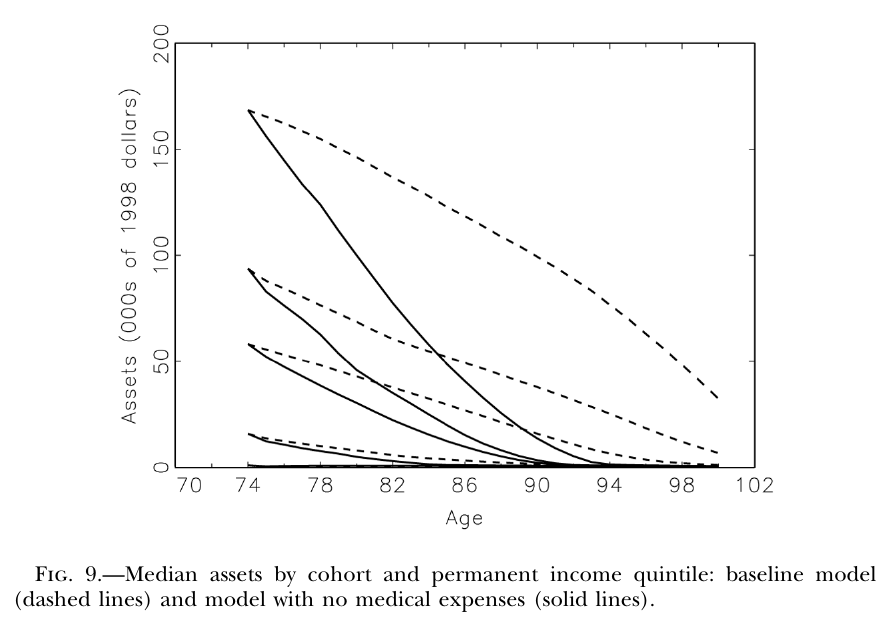
\includegraphics[width=0.6\textwidth]{./OriginalTablesFigures/DFJ2010_Figure9.png} \\
\includegraphics[width=0.7\textwidth]{../SavedOutput/Graphs/DFJ2010_Fig9_nomedex.png}
\caption{DFJ2010 Figure 9: Original (top) and replication (bottom). Baseline (dashed) versus no medical expenses (solid). DFJ2010: with no out-of-pocket medical expenses the top quintile ``would deplete their net worth by age 94'', whereas in the baseline ``at age 100, they keep almost \$40,000''. Here the top quintile's median is \$1,000 at 94 with no medical expenses, and \$36,000 at 100 in the baseline (\$83,000 at 94).}\label{fig:dfj9}
\end{figure}

\begin{figure}[htbp]
\centering
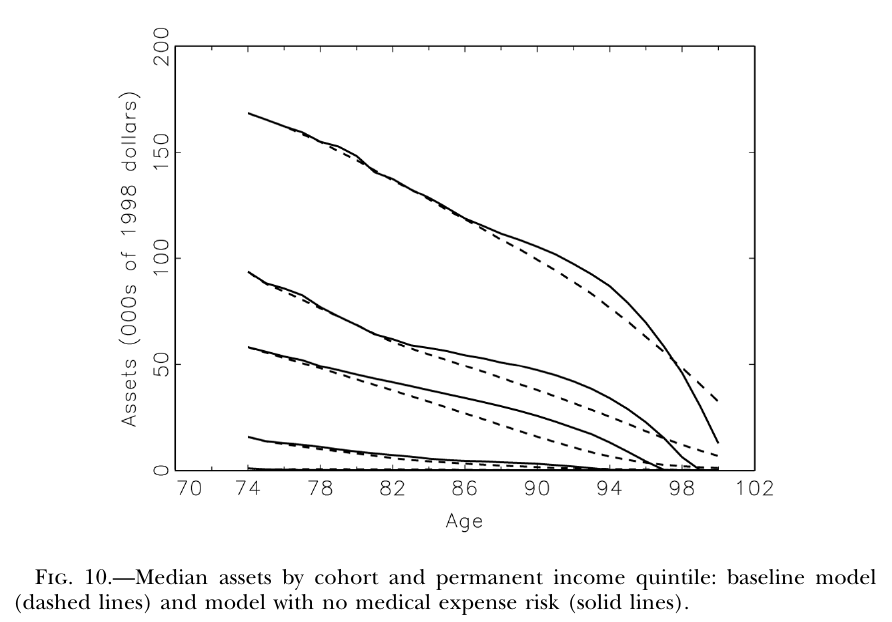
\includegraphics[width=0.6\textwidth]{./OriginalTablesFigures/DFJ2010_Figure10.png} \\
\includegraphics[width=0.7\textwidth]{../SavedOutput/Graphs/DFJ2010_Fig10_nomedexrisk.png}
\caption{DFJ2010 Figure 10: Original (top) and replication (bottom). Baseline (dashed) versus no medical-expense risk with the same conditional mean (solid). DFJ2010 find ``only a small effect on the profiles of median wealth'', and sometimes an increase in assets, because fewer catastrophic expenses means less of the expense is covered by the floor. Here the effect is larger than theirs: removing the risk while keeping the mean \emph{raises} the top quintile's median at 90 from \$108,000 to \$132,000 and the fourth quintile's from \$37,000 to \$54,000, for the reason DFJ2010 give (with no upper tail, none of the expense is picked up by the floor, so the expected out-of-pocket burden at old ages is higher), and then all quintiles run their assets down to zero by 100, because with certain expenses there is nothing left to insure against at the end.}\label{fig:dfj10}
\end{figure}

\begin{figure}[htbp]
\centering
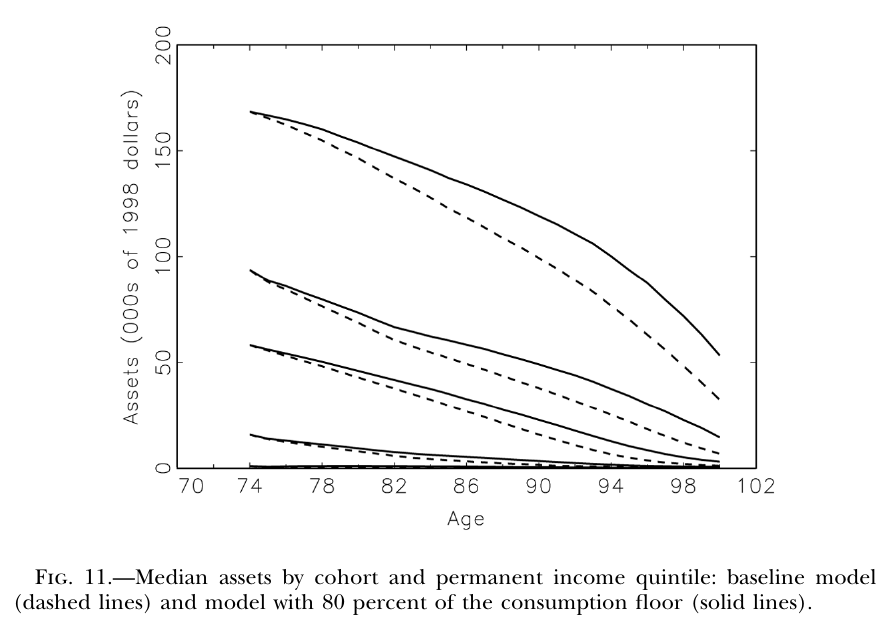
\includegraphics[width=0.6\textwidth]{./OriginalTablesFigures/DFJ2010_Figure11.png} \\
\includegraphics[width=0.7\textwidth]{../SavedOutput/Graphs/DFJ2010_Fig11_cfloor80.png}
\caption{DFJ2010 Figure 11: Original (top) and replication (bottom). Baseline (dashed) versus a consumption floor at 80 percent of its value (solid). DFJ2010: the assets of 90-year-olds in the top quintile rise from \$100,000 to \$120,000 and in the fourth quintile from \$40,000 to \$50,000, so ``the consumption floor thus matters for wealthy individuals as well as poor ones''. Here: top quintile at 90 from \$108,000 to \$130,000, fourth from \$37,000 to \$50,000, third from \$16,000 to \$23,000; the paper's numbers almost exactly.}\label{fig:dfj11}
\end{figure}

\section{The model with endogenous medical expenses}\label{sec:endog}
Section IX of DFJ2010 replaces the exogenous medical-expense process with a model in which medical goods are chosen, so that the medical-expense risk is a risk to the marginal utility of medical goods rather than to the budget directly. This section records how that model is expressed in the toolkit, the targets it is estimated on, its fit at DFJ2010's published parameters, and the estimates. Its figures are DFJ2010's Figures 12--14 and A4: Figures 12 and A4 at the published parameters (Figures \ref{fig:em12} and \ref{fig:emA4}) and at the estimates (Figures \ref{fig:em12est} and \ref{fig:emA4est}), and the counterfactual Figures 13 and 14 at the estimates (Figures \ref{fig:em13} and \ref{fig:em14}).

\subsection{The model}
Per-period utility is (DFJ2010 eqn 21)
\begin{equation*}
 u(c,m)=\frac{c^{1-\nu}}{1-\nu}+\mu(j,h,\zeta,\xi)\,\frac{m^{1-\omega}}{1-\omega}, \qquad \ln\mu = D(j,h,male)+\sigma(j,h,male)\,(\zeta+\xi),
\end{equation*}
where $m$ is total medical goods and $\mu$ is the medical-needs shifter. The shifter's mean $D$ and the standard deviation $\sigma$ of its shock are cubic and quadratic polynomials in age with bad-health and male terms (24 coefficients, \texttt{mxvec} in \texttt{singlsav51\_wave8.gau}; the permanent-income terms are fixed at zero, as the paper says). The shock $\zeta+\xi$ has unit variance, with $\zeta$ an AR(1) of autocorrelation $0.849$ carrying $48.8$ percent of the variance and $\xi$ i.i.d.\ (the exogenous model: $0.922$ and $33.5$ percent). The budget constraint is (eqn 24)
\begin{equation*}
 a'=a+aftertaxincome+govtransfers-c-q(j,h)\,m, \qquad a'\geq 0,
\end{equation*}
with $q(j,h)$ the out-of-pocket share (the coinsurance rate, \texttt{medpriceprof.out}: $q=\exp(b_0(j)+b_1(j)\,bad)$, falling with age and in bad health; the male coefficient is zero at every age). The consumption floor becomes a utility floor $u_{min}$: the transfer is $\max(0,x_{min}(\mu,q)-x)$ where $x$ is cash on hand and $x_{min}$ the least spending that reaches $u_{min}$ at the optimal split; when it is positive the household saves nothing. DFJ2010 index the floor by $eMin$, the consumption level that delivers $u_{min}$ when $\mu=1$ (their Table A1 footnote; the C code's \texttt{uMin=getUtility(eMin,eMin,1)}). The estimated endogenous model has no bequest motive and no health shifter of utility. Everything else (health, survival, income, taxes, the ten permanent types) is as in Section \ref{sec:model}. The published parameters are Table A1 column 5 of the online appendix: $\nu=2.146$, $\omega=3.191$, $\beta=0.990$, $eMin=\exp(5.30863)=202$.

\subsection{No decision variable is needed}
The natural toolkit formulation adds $m$ as a decision variable on a grid. It is not needed: the intratemporal first-order condition $c^{-\nu}=(\mu/q)\,m^{-\omega}$ gives $m=(\mu/q)^{1/\omega}c^{\nu/\omega}$, so for given $(a',a,h,\zeta,\xi,j)$ the split of total spending $s=x-a'$ between $c$ and $qm$ is the root of $c+q(\mu/q)^{1/\omega}c^{\nu/\omega}=s$, which is monotone in $c$. The return function finds it by bisection (42 fixed steps, as the GPU needs a data-independent loop; DFJ2010's C code does the same), and finds $x_{min}$ by a second bisection on $u(c,m(c))=u_{min}$. The model therefore keeps the exogenous model's state space (420,420 points per age) and its single choice $a'$; the value function takes 110 seconds for the ten types against 20 for the exogenous model. For comparison, part 9 of the script solved the same model with $m$ on a 101-point decision grid: it does not fit in the 42 GB of GPU memory without looping over the i.i.d.\ shock, and with that loop it takes 8,596 seconds, 78 times the bisection.

Out-of-pocket medical expenses, the object the data measure, are $qm$; they are a function of the state and the policy, so every statistic of them comes from the agent distribution without simulation. DFJ2010 bottom-code medical expenses at \$250 (\texttt{minmedex} in \texttt{singlsav51\_wave8.gau}, applied in \texttt{gmmcrit51.g} to the two-year average, in the data and in the simulation alike; neither the paper nor the supplemental appendix gives a reason, and the evident one is that the autocorrelation moments are of logs, so a wave with no out-of-pocket spending would otherwise be minus infinity). The toolkit's window statistics average the raw function, so the replication floors each year at \$125 instead: the two agree whenever both years are at or above \$250, and differ by at most a factor of two in the floored value when a year is below it, which in the model is a low-need draw and in the data a wave with little or no spending.

\subsection{Targets}
DFJ2010's criterion (their online appendix A.2) adds to the asset medians, for each cohort, permanent-income half and year 1998--2006, the mean of out-of-pocket medical expenses, the 90th percentile as an indicator moment, and the first and second autocorrelations of log medical expenses, for 249 moments. All three medical-expense blocks are of two-year averages: \texttt{gmmcrit51.g} averages adjacent years, in the data and in the simulation alike, before taking means, percentiles and autocorrelations. The data cells are built in \texttt{DFJ2010\_DataWork.m} with the same 500-resample bootstrap as the asset medians (and checked against DFJ2010's own extract, where the same rules give their cell counts).

The replication computes the model moments the same way, with the toolkit's window statistics (\texttt{simoptions.ntimeperiods=2}): the mean and the 90th percentile of the two-year average come from the life-cycle profiles, and the correlations of the log two-year average at horizons of two and four years from the autocorrelation command, which carries the joint distribution over the four consecutive ages that a pair of windows spans. That gives 252 moments: the 102 asset medians, 45 means, 45 90th percentiles, 35 first and 25 second autocorrelations. The 20 autocorrelations that pair a wave with the 1996 wave (the first autocorrelation in 1998 and the second in 2000, for each cohort and permanent-income half) are not targeted. In the model each cohort enters at its 1996 age, so the 1996 wave, the average of 1995 and 1996, would start a year before the cohort is in the model. DFJ2010's simulation is annual and does not simulate the 1996 wave either: each simulated person starts from a person in the 1996 data, and in \texttt{gmmcrit51.g} the simulated panel's 1996 wave is that person's observed 1996 value, the survey's own average over 1995 and 1996, placed in front of the simulated two-year averages. Their simulation draws the starting medical-needs shock independently of that observed value (\texttt{initmx} in \texttt{getdat50\_wave8.g}). So in their criterion these 20 moments correlate a model draw with an observed number, which are related only through the observables they share (age, health, sex and permanent income) and not through the persistent shock that the other autocorrelations measure. Reproducing them here would mean adding the 1996 expense to the cohorts' entry state; the replication does not do this. The 90th percentile is calculated differently from DFJ2010's. Their moment condition (online appendix eqn A2) is an indicator moment: in each cell, the share of the data observations at or below the model's 90th percentile should be 0.9, $E[\mathbb{I}\{m_{it}\leq m^{90}_{pqt}(\Delta)\}-0.9]=0$, the same form as their median conditions. The replication targets the level instead: the model's 90th percentile against the data's, each squared gap weighted by the inverse bootstrap variance of the data percentile. The two agree when the model's percentile equals the data's, but weight a misfit differently, exactly as for the medians (Appendix \ref{app:medianmoments}); the replication does not implement the indicator form for the 90th percentile. It is computed with the toolkit's one-pass t-digest (\texttt{simoptions.windowmethod='tdigest1'}): the exact enumeration ran out of memory in the estimation, and at the published parameters the approximation moves the objective by 0.3. The lower half of the permanent-income distribution is quintiles 1 and 2 and the upper half quintiles 3 to 5 (the quintile types sit at the 10th, 30th, \dots, 90th percentiles, and the paper's $(q-1)/Q\leq I<q/Q$ puts the 50th in the upper half).

Two conventions differ from DFJ2010's. Their autocorrelations centre and scale each date's log expenses by the full cell's mean and standard deviation, over the people observed at both dates; the toolkit's autocorrelation command computes the ordinary correlation of the pair population, with its own means and standard deviations. The data moments are computed in both definitions (\texttt{DFJ2010\_MedexTargets.m}, rows \texttt{ac1}/\texttt{ac2} and \texttt{ac1dfj}/\texttt{ac2dfj}, each with its own bootstrap), and the estimation is run on each: on the toolkit definition through the AutoCorr targets (part 7 of the script), and on DFJ2010's through \texttt{estimoptions.CustomModelStats} (part 8). And the weighting matrix is diagonal with the bootstrap variances, as for the asset medians. Both are choices of the replication, not of the paper.

\begin{sloppypar}
The autocorrelations are computed without any panel simulation. The toolkit's \texttt{EvalFnOnAgentDist\_\allowbreak AutoCorrTransProbs\_FHorz} pushes the age-$j$ distribution forward through the policy and the shock transitions (the two-step push of \citet{Tan2020}) to obtain the joint distribution of a function at ages $j$ and $j+k$; for this replication it acquired exact horizons (\texttt{simoptions.timehorizons}), multi-period windows and their logs (\texttt{simoptions.ntimeperiods}, \texttt{logwhichcombos}), conditional restrictions on the origin state, a permanent-type wrapper, and a target type \texttt{TargetMoments.AutoCorr.cohortC.\allowbreak restriction.fn\_2periodAverage\_log.\allowbreak AutoCorrelation\_horizonK} in the cohort estimator. The targets are therefore exact functions of the parameters, with no simulation noise in the objective.
\end{sloppypar}

\subsection{Fit at the published parameters}
At DFJ2010's published parameters the objective over the 252 moments is 866.3 with the autocorrelations in the toolkit's definition and 799.1 in DFJ2010's (their own criterion gives 667 on 242 degrees of freedom: the paper's endogenous model is rejected, and that is reproduced). The estimation command evaluated once at those parameters, with \texttt{estimoptions.skipestimation} and \texttt{skipjacobian}, gives the same two numbers to within $10^{-12}$, so the targets the estimator stacks are the ones described here. By block: the asset medians contribute 225.3 (against 115.5 for the exogenous benchmark at its published parameters, so the endogenous model fits assets visibly worse, as in the paper), the medical-expense means 159.3, the 90th percentiles 322.0, the first autocorrelations 119.0 (61.9 in DFJ2010's definition) and the second 40.6 (30.6). The mean out-of-pocket expense over the 45 cells is \$4,362 in the model against \$4,267 in the data, with a correlation of cell means of 0.85. The 90th percentile averages \$9,800 against \$11,600: the model's upper tail is too thin, and it is the largest block. For the first cohort the model's first autocorrelations are 0.43--0.48 against 0.48--0.63 in the data, and the second 0.32--0.36 against 0.31--0.55. On the earlier annual-lag criterion the model's first autocorrelations were 0.29--0.35, so computing them on two-year averages, as DFJ2010 do, closes most of that gap. Figures \ref{fig:em12} and \ref{fig:emA4} show the asset and medical-expense fit.

\begin{figure}[htbp]
\centering
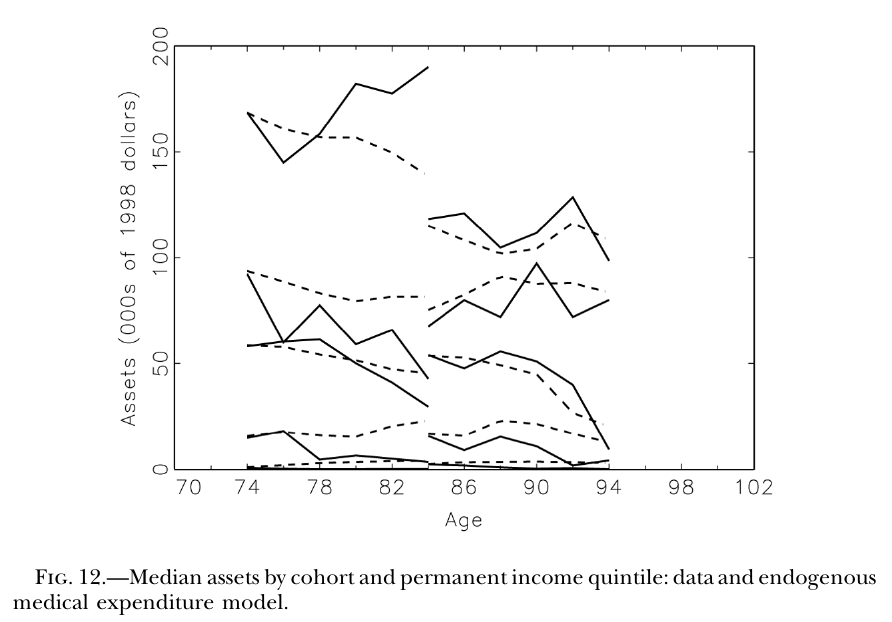
\includegraphics[width=0.55\textwidth]{./OriginalTablesFigures/DFJ2010_Figure12.png} \\
\includegraphics[width=0.75\textwidth]{../SavedOutput/Graphs/DFJ2010_EM_Fig12_assets.png}
\caption{DFJ2010 Figure 12: Original (top) and replication (bottom). Median assets by cohort and permanent-income quintile, data (solid) and the endogenous medical-expense model at its published parameters (dashed), for the cohorts aged 74 and 84 in 1996, 1996--2006. The asset block of the objective, over all five cohorts, is 225.3 here against 115.5 for the exogenous benchmark.}\label{fig:em12}
\end{figure}

\begin{figure}[htbp]
\centering
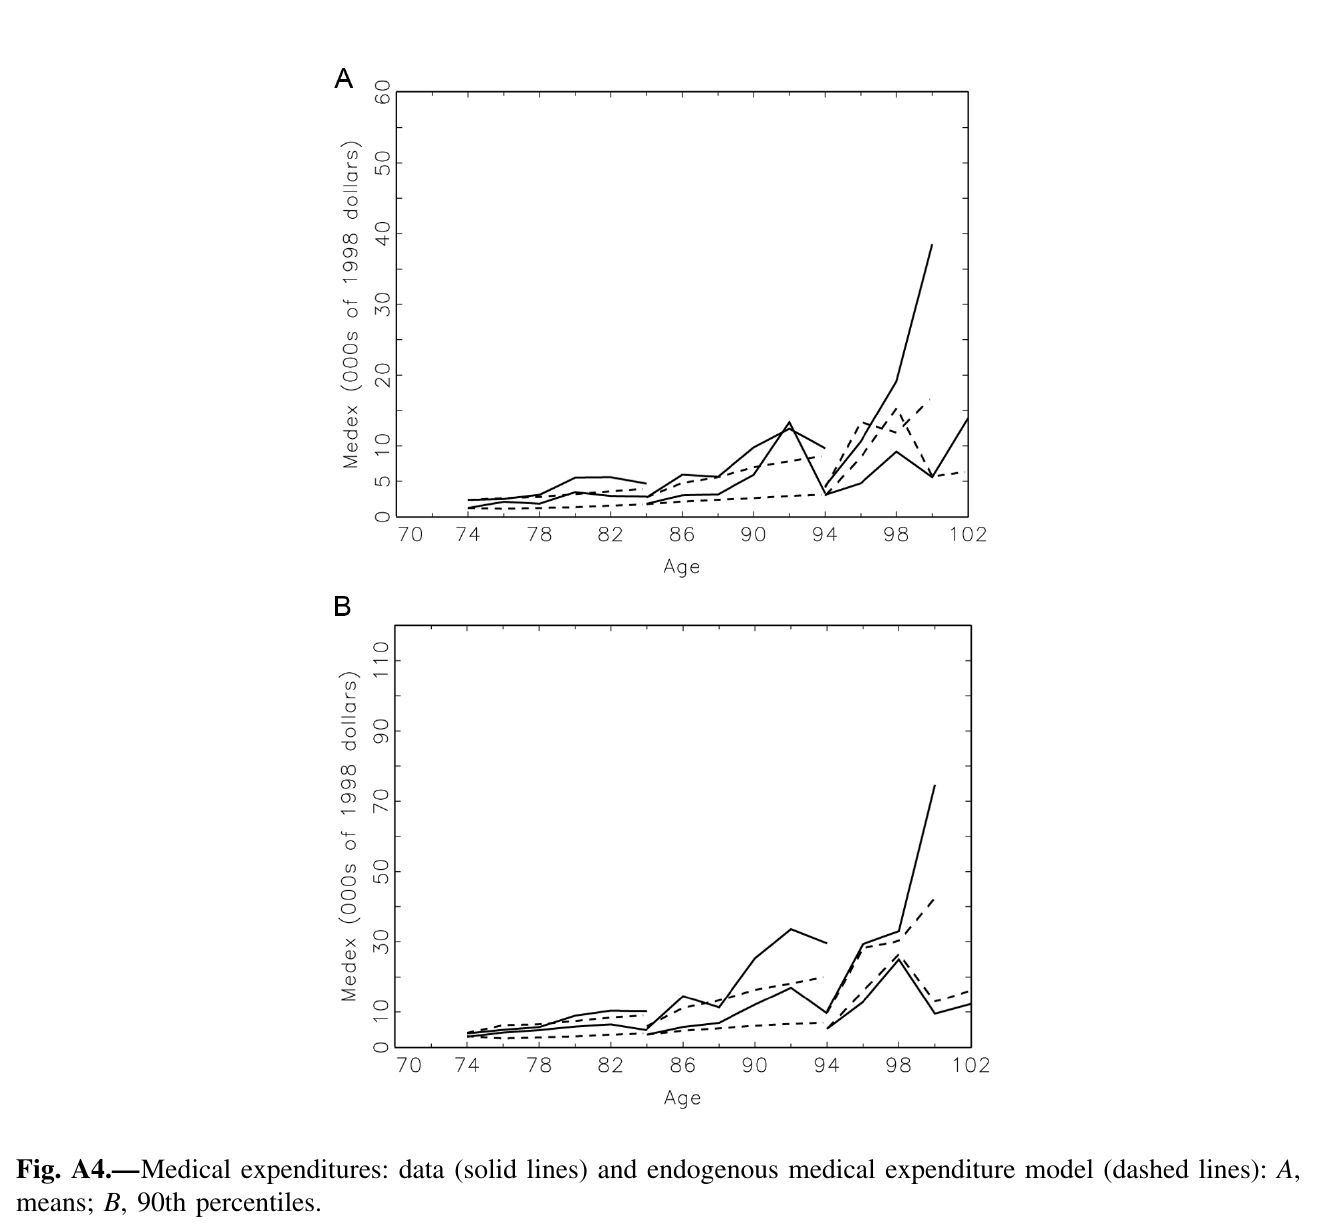
\includegraphics[width=0.5\textwidth]{./OriginalTablesFigures/DFJ2010_FigureA4.png} \\
\includegraphics[width=0.85\textwidth]{../SavedOutput/Graphs/DFJ2010_EM_FigA4_medex.png}
\caption{DFJ2010 Figure A4: Original (top) and replication (bottom). Mean (top) and 90th percentile (bottom) of out-of-pocket medical expenses by cohort and permanent-income half, data (solid) and the endogenous model at its published parameters (dashed), ages on the horizontal axis so that each cohort is one line segment.}\label{fig:emA4}
\end{figure}

\clearpage
\subsection{Estimation}
Parts 7 and 8 of the script run the estimation, with the autocorrelation targets in the toolkit's definition and in DFJ2010's respectively. Part 8 goes through \texttt{estimoptions.CustomModelStats}, which the cohort estimator calls once per cohort on that cohort's distribution; \texttt{DFJ2010\_EM\_CustomStats.m} forms DFJ2010's full-cell-normalised correlation from the autocorrelation command's pair covariance, pair means and cell means and standard deviations, so no simulation is involved in either. The four preference and floor parameters $\nu$, $\omega$, $\beta$ and $eMin$ are estimated by \texttt{lsqnonlin} from the published values, with the 24 shifter coefficients held at DFJ2010's estimates (DFJ2010 estimate those jointly; making them estimable needs a mapping from the coefficients to the per-type age profiles, which the toolkit's \texttt{ParametrizeParamsFn} provides but which is not wired here). The standard errors use the largest finite-difference step, as for the exogenous model, since the asset medians sit on a grid. Table \ref{tab:endog} gives the estimates in both definitions.

The estimation in DFJ2010's definition was run twice. The first run started from the published values and \texttt{lsqnonlin} stopped on its step-size tolerance after 80 evaluations, at an objective of 552.4, but the cluster's 24-hour limit ended the job while it was computing the standard errors, so nothing was saved. The second run started from the point where the first had stopped. \texttt{lsqnonlin} found no better point within its tolerance in 55 evaluations and returned that point, and the run then computed the standard errors. The estimates in Table \ref{tab:endog} are therefore those of a minimisation from the published values, with the standard errors from the second run.

\begin{table}[htbp]
\centering
\caption{The endogenous medical-expense model: DFJ2010's estimates (their Table A1 column 5, whose original is in Table \ref{tab:tableA1}) and the replication in both definitions of the autocorrelations}\label{tab:endog}
\small
\begin{tabular}{lccc}
\toprule
 & & \multicolumn{2}{c}{This replication, autocorrelations in} \\
\cmidrule(lr){3-4}
 & DFJ2010 & the toolkit's definition & DFJ2010's definition \\
\midrule
$\nu$ & 2.15 (.055) & 1.84 (.080) & 1.90 (.082) \\
$\omega$ & 3.19 (.054) & 3.03 (.073) & 3.09 (.075) \\
$\beta$ & .99 (.01) & .997 (.011) & .995 (.011) \\
$eMin$ & 202 (23.4) & 247 (47) & 263 (64) \\
objective & 667.0 [242] & 618.1 [248] & 552.5 [248] \\
\midrule
\multicolumn{4}{l}{\textit{Replication objective by block, at the published parameters / at the estimates}} \\
asset medians (102) & & 225.3 / 151.4 & 225.3 / 152.4 \\
mean medical expenses (45) & & 159.3 / 120.8 & 159.3 / 120.5 \\
90th percentiles (45) & & 322.0 / 187.7 & 322.0 / 187.2 \\
first autocorrelations (35) & & 119.0 / 115.9 & 61.9 / 61.1 \\
second autocorrelations (25) & & 40.6 / 42.3 & 30.6 / 31.2 \\
\bottomrule
\end{tabular}
\par\smallskip
\begin{minipage}{0.95\textwidth}\footnotesize
Standard errors in parentheses, degrees of freedom in brackets. DFJ2010 estimate 7 parameters on 249 moments, with the 90th percentile as an indicator moment; the replication estimates 4 on 252, with the 90th percentile as a level and the shifter coefficients fixed, so its objectives are not on the same criterion as theirs. The two replication columns differ only in how the autocorrelations are centred and scaled, in the data and in the model. On an A100, the toolkit-definition estimation took 1,277 minutes: about 75 objective evaluations in the minimisation and 36 for the standard errors, of about 11.5 minutes each (value function 100--180 seconds; for the five cohorts together, distributions 45 seconds, window statistics 410 seconds and autocorrelations 130 seconds). The DFJ2010-definition estimation took about 12.5 minutes per evaluation: 80 evaluations in the first run, and 55 plus 36 for the standard errors in the second (1,087 minutes).
\end{minipage}
\end{table}

The estimation lowers the objective from 866 to 618 in the toolkit's definition, and from 799 to 552 in DFJ2010's. Most of the gain is in the asset medians (225 to 151) and the 90th percentiles (322 to 188), with the means improving less (159 to 121). The autocorrelations barely move (119 to 116 and 41 to 42), which suggests that they are governed by the shock process, held fixed here, rather than by the four estimated parameters. In the toolkit's definition the estimates are close to DFJ2010's. $\beta$ and $eMin$ are within one of the replication's standard errors of DFJ2010's values ($eMin$ is about two of DFJ2010's own, which are half as wide). $\omega$ is 3.03 against 3.19, and $\nu$ 1.84 against 2.15, about two and four of the replication's standard errors below. This is a change from the earlier annual-lag criterion, which gave $\nu=3.29$, $\omega=4.38$, $\beta=.963$ and $eMin=\$1{,}397$: there the model's autocorrelations were well below the data's, and the minimiser raised both curvature parameters to make the medical-expense choice more persistent. On two-year windows, as DFJ2010 compute them, the model's autocorrelations are near the data's at the published parameters, and that push disappears. The two caveats of Section \ref{sec:results} apply here too: the asset medians sit on the grid, and $eMin$ is identified mainly by the bottom-quintile cells.

With the autocorrelations in DFJ2010's definition the estimates move a little further towards theirs: $\nu$ 1.90 and $\omega$ 3.09, about three and 1.4 of the replication's standard errors below DFJ2010's values, with $\beta$ and $eMin$ again within one. The two replication columns are within one standard error of each other for every parameter. The lower objective in DFJ2010's definition comes almost entirely from the autocorrelation blocks (92 against 158 at the estimates), which fit better in that definition both at the published parameters and at the estimates (92 against 160 at the former); the other three blocks are nearly identical in the two columns. As in the toolkit's definition, the autocorrelation blocks barely change between the published parameters and the estimates.

What remains different from the paper: the 90th percentile as an indicator rather than a level, the 20 autocorrelations with the 1996 wave, and the joint estimation of the shifter coefficients. Each is a convention of the moments or of the estimation rather than of the model.

\subsection{Fit and counterfactuals at the estimates}
Part 10 of the script solves the endogenous model at the estimates with the autocorrelations in DFJ2010's definition and redraws Figures 12 and A4 there (Figures \ref{fig:em12est} and \ref{fig:emA4est}). The asset block of the objective it computes from the redrawn medians is 152.4, the value the estimation reports, so the figures are of the estimated model. The asset fit improves visibly on the published parameters (Figure \ref{fig:em12}). The medical-expense fit moves the other way in levels: averaged over the 45 cells, the model's mean is \$3,547 against \$4,267 in the data and its 90th percentile \$7,906 against \$11,633, with two thirds of the cells below the data, the largest gaps in the upper half of the permanent-income distribution after age 95. The objective still falls in both blocks, because the cells the estimates fit worse are the imprecisely measured ones: the mean standardised gap falls from 1.42 to 1.36 for the means and from 1.77 to 1.53 for the 90th percentiles. DFJ2010's appendix makes the same observation of their own estimates, that the model slightly underpredicts medical expenditures.

The two counterfactuals of Section IX follow Section \ref{sec:results}'s Figures 9--11: the cohort aged 74 in 1996, followed to age 100 with no attrition, the policy solved with mortality risk at the estimates. Setting the medical-needs shifter to zero, as DFJ2010 do to eliminate medical expenses, makes every quintile run its assets down (Figure \ref{fig:em13}): the top quintile's median at 90 falls from \$56,000 to \$6,000 and is essentially zero by 92, the same conclusion as in the exogenous model (Figure \ref{fig:dfj9}). Halving the floor raises the savings of every quintile in both models, and by much less in the endogenous one (Figure \ref{fig:em14}): the top quintile's median at 90 rises from \$108,000 to \$179,000 in the exogenous model and from \$56,000 to \$70,000 in the endogenous one. DFJ2010 attribute the smaller response to the extra margin the endogenous model gives, since retirees can cut medical spending as well as consumption. In the endogenous model the floor is indexed by $eMin$, and halving it follows their footnote 8; in the exogenous model it is the consumption floor at DFJ2010's Table 3 column 1 value, as in Figures 9--11.

The endogenous baseline holds less wealth late in life than the exogenous one, \$56,000 at 90 in the top quintile against \$108,000. The two baselines are at different parameters: the exogenous model at DFJ2010's published benchmark, the endogenous one at the replication's estimates. So the gap between them is not a comparison of the two medical-expense mechanisms alone.

\begin{figure}[htbp]
\centering
\includegraphics[width=0.75\textwidth]{../SavedOutput/Graphs/DFJ2010_EM_Fig12_assets_estimates.png}
\caption{DFJ2010 Figure 12 at the estimates, replication only (DFJ2010's original is above Figure \ref{fig:em12}; autocorrelations in DFJ2010's definition): median assets by cohort and permanent-income quintile, data (solid) and model (dashed), for the cohorts aged 74 and 84 in 1996, 1996--2006. The asset block of the objective, over all five cohorts, is 152.4, against 225.3 at the published parameters (Figure \ref{fig:em12}).}\label{fig:em12est}
\end{figure}

\begin{figure}[htbp]
\centering
\includegraphics[width=0.95\textwidth]{../SavedOutput/Graphs/DFJ2010_EM_FigA4_medex_estimates.png}
\caption{DFJ2010 Figure A4 at the estimates, replication only (DFJ2010's original is above Figure \ref{fig:emA4}): mean (top) and 90th percentile (bottom) of out-of-pocket medical expenses by cohort and permanent-income half, data (solid) and model (dashed). The model is below the data in two thirds of the cells, most in the upper half after age 95.}\label{fig:emA4est}
\end{figure}

Figure \ref{fig:dfjA2} is the appendix's Figure A2: the distribution of out-of-pocket medical expenses in the data against both models, the exogenous one at DFJ2010's benchmark and the endogenous one at the estimates. As in the moments, both sides are two-year averages bottom-coded at \$250, pooled over the cohort, permanent-income half and wave cells with the data's cell counts as weights, and the model's expenses are net of the government transfer. In panel A the model's CDF lies above the data's up to about \$40,000, so the exogenous model puts too little weight on large expenses: 59 percent of its expenses are below \$1,000 against 49 percent in the data, and 92 against 88 percent below \$5,000. DFJ2010 find the same of their exogenous model, and attribute it to the exogenous process being estimated on expenses net of Medicaid. The endogenous model, whose expenses are net of the transfer by construction, is closer at every level: 53 percent below \$1,000, and within two percentage points of the data from \$5,000 up. DFJ2010 find that theirs understates the probability of low expenses and fits the upper tail from about \$20,000; here the small gap at the bottom goes the other way, with slightly too much mass below \$1,000.

\begin{figure}[htbp]
\centering
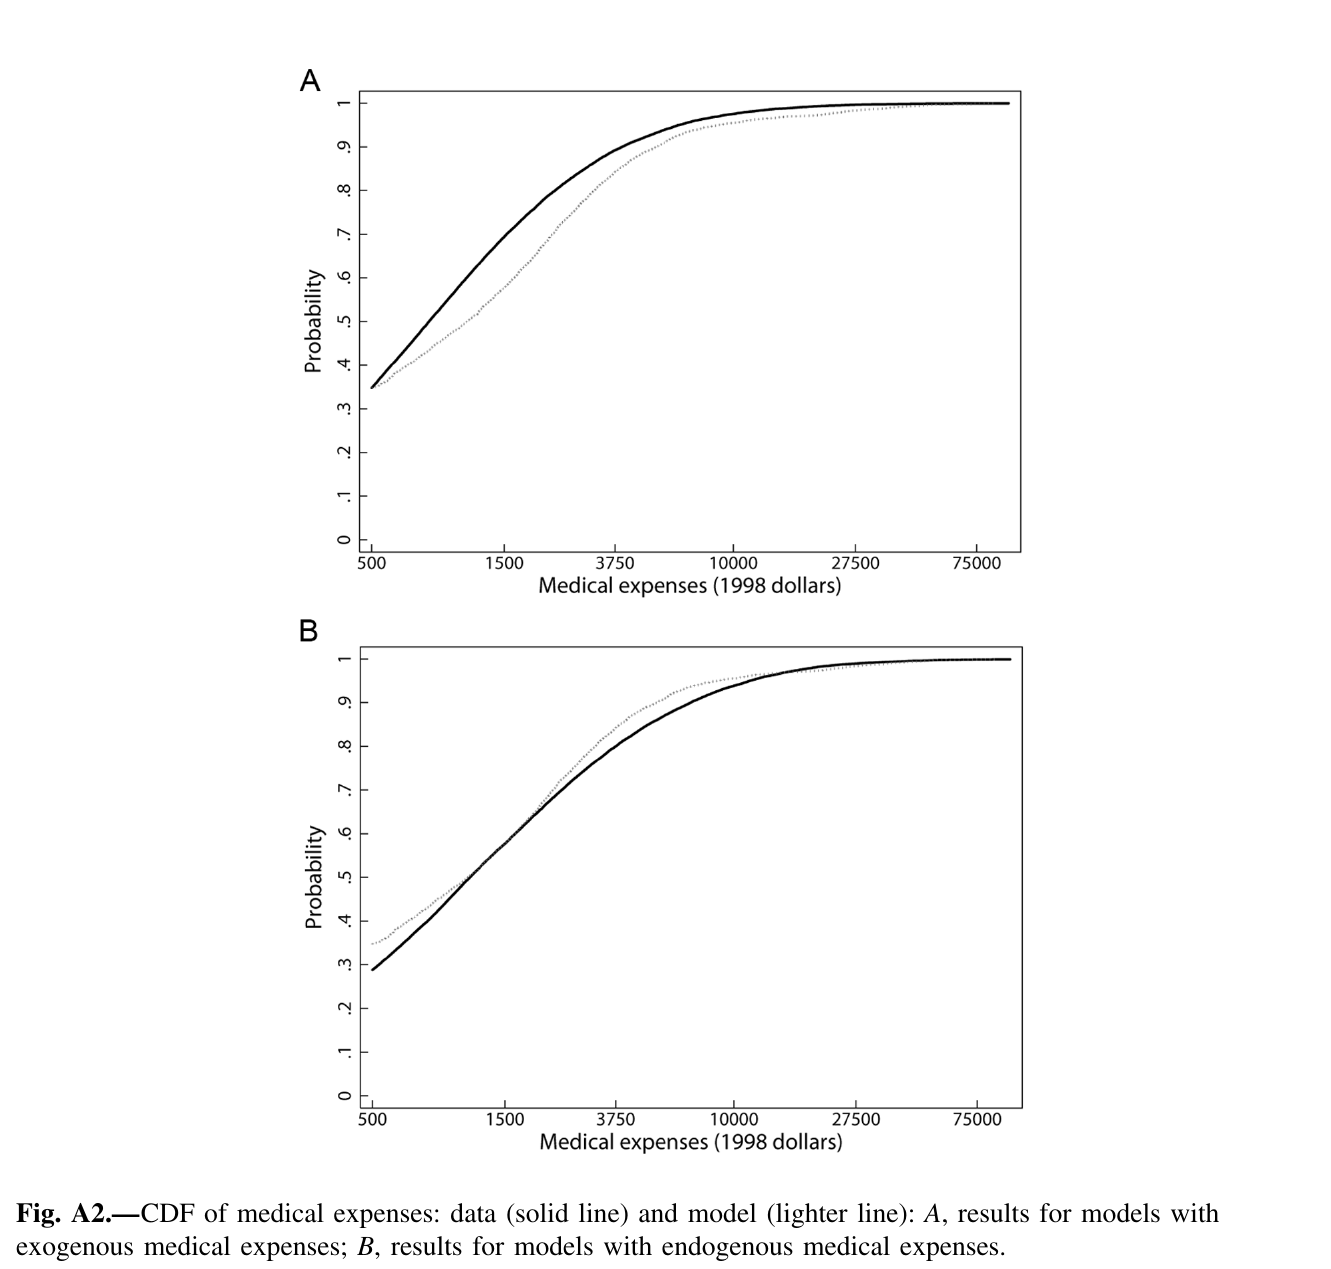
\includegraphics[width=0.55\textwidth]{./OriginalTablesFigures/DFJ2010_FigureA2.png} \\
\figfile{../SavedOutput/Graphs/DFJ2010_FigA2_medexCDF.png}{0.85}
\caption{DFJ2010 appendix Figure A2: Original (top) and replication (bottom). CDF of out-of-pocket medical expenses, two-year averages in the 1998--2006 waves, data (solid) and model (dashed). A: the exogenous model at DFJ2010's Table 3 column 1, expenses net of government transfers. B: the endogenous model at the estimates (autocorrelations in DFJ2010's definition).}\label{fig:dfjA2}
\end{figure}

\begin{figure}[htbp]
\centering
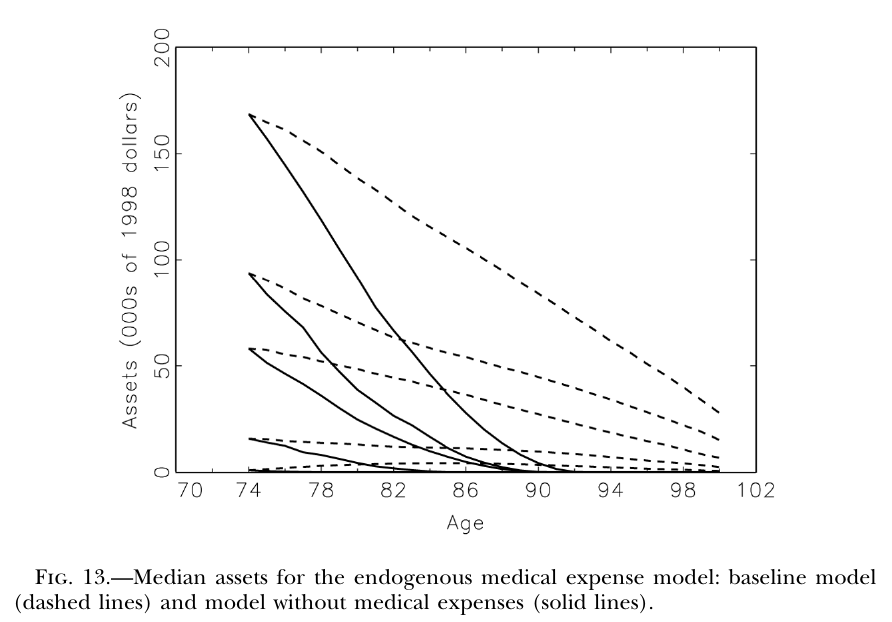
\includegraphics[width=0.6\textwidth]{./OriginalTablesFigures/DFJ2010_Figure13.png} \\
\includegraphics[width=0.7\textwidth]{../SavedOutput/Graphs/DFJ2010_EM_Fig13_nomedex.png}
\caption{DFJ2010 Figure 13: Original (top) and replication (bottom). The endogenous model at the estimates, baseline (dashed) versus no medical expenses (solid, the medical-needs shifter set to zero), median assets by permanent-income quintile for the cohort aged 74 in 1996 with no attrition. The top quintile's median at 90 is \$56,000 in the baseline and \$6,000 without medical expenses.}\label{fig:em13}
\end{figure}

\begin{figure}[htbp]
\centering
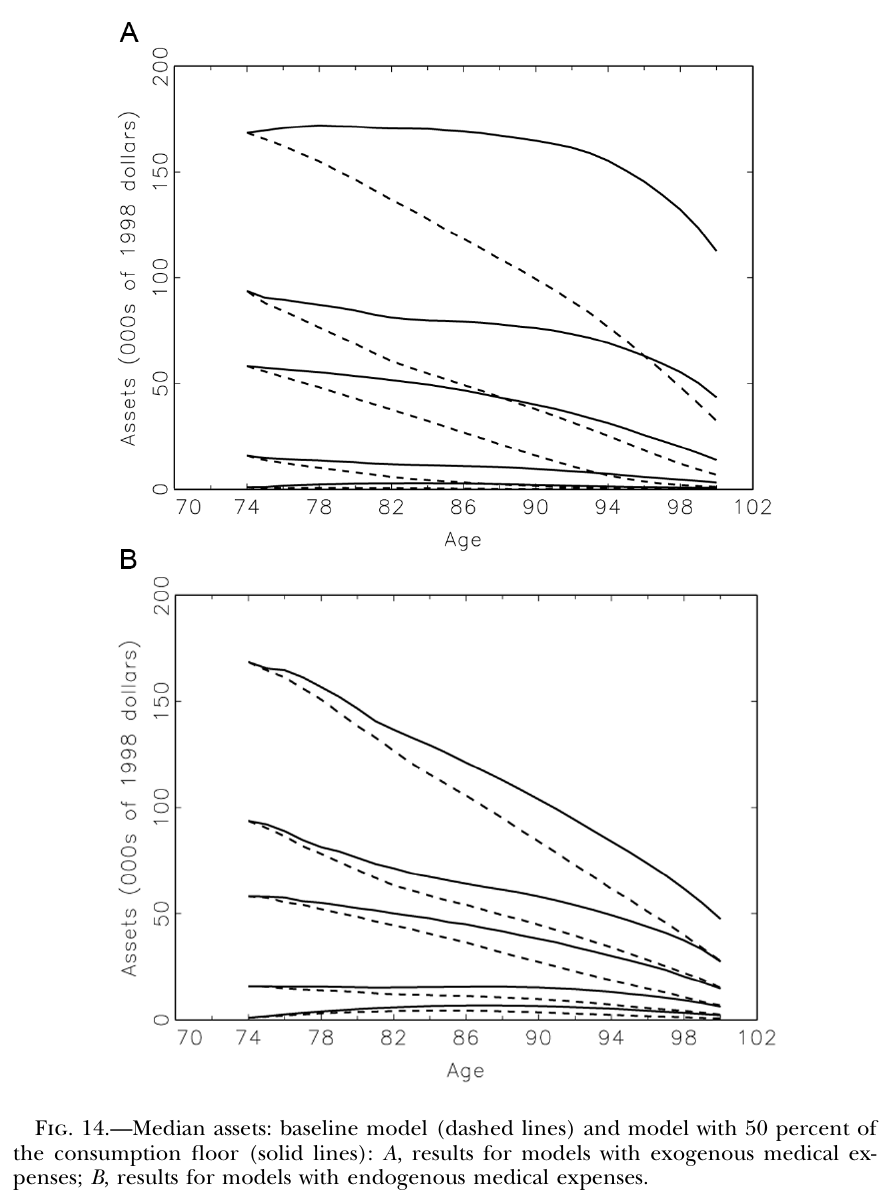
\includegraphics[width=0.42\textwidth]{./OriginalTablesFigures/DFJ2010_Figure14.png} \\
\includegraphics[width=0.85\textwidth]{../SavedOutput/Graphs/DFJ2010_Fig14_cfloor50.png}
\caption{DFJ2010 Figure 14: Original (top) and replication (bottom). Baseline (dashed) versus 50 percent of the floor (solid), median assets by permanent-income quintile for the cohort aged 74 in 1996 with no attrition. A: the exogenous model at DFJ2010's Table 3 column 1, the consumption floor halved. B: the endogenous model at the estimates, $eMin$ halved. The top quintile's median at 90 rises from \$108,000 to \$179,000 in A and from \$56,000 to \$70,000 in B.}\label{fig:em14}
\end{figure}

\clearpage
\appendix
\section{Median-based moment conditions: DFJ2010 versus VFI Toolkit}\label{app:medianmoments}

Consider one cell: cohort $p$, permanent-income quintile $q$, calendar year $v$. Let $m^d_{pqv}$ be the median of assets among the data observations in the cell (individuals alive in $v$), and let $\hat{a}_{pqv}(\Delta)$ be the median of assets in the same cell in the model, which depends on the parameters $\Delta$ being estimated.

\paragraph{What DFJ2010 do.}
Their moment condition (their eqn 18) is
\begin{equation*}
 E\left[ \mathbb{I}\{a_{iv} \leq \hat{a}_{pqv}(\Delta)\} - \tfrac{1}{2} \,\middle|\, p,q,v,\ i \text{ alive at } v \right] = 0 .
\end{equation*}
The sample analogue is the share of data observations in the cell whose assets lie at or below the model's median, minus one half. At the true parameters that share is exactly one half, so the model median equals the data median. In that sense they ``match medians'', but the moment itself is a probability, not a dollar amount.

Two properties follow. First, the moment is bounded in $[-\tfrac{1}{2},\tfrac{1}{2}]$ in every cell, so a cell in which the model is wildly off contributes at most $\tfrac{1}{4}$ to the (unweighted) criterion whether the cell's median is \$500 or \$200,000. Second, the variance of the moment is approximately $1/(4 n_{pqv})$, so the efficient weighting matrix depends only on cell sizes (and, off the diagonal, on the overlap of individuals across years); no dollar units enter. The cost is that the moment function is a step function of $\Delta$: it is not differentiable, so DFJ2010 have to obtain the Jacobian and the standard errors by the Pakes--Pollard route, which needs a kernel-density estimate $f_{pqv}(m)$ of the asset density at the median (see their online appendix; the GAUSS code calls Koning's kernel routine).

\paragraph{What VFI Toolkit does.}
The toolkit's \texttt{EstimateLifeCycleModel\_PType\_MethodOfMoments} takes a target statistic and compares it with the same statistic in the model. With the median of assets as the target the moment is
\begin{equation*}
 \hat{a}_{pqv}(\Delta) - m^d_{pqv} ,
\end{equation*}
in dollars. The data medians (and their bootstrap covariance) are computed once, before estimation, by \texttt{DFJ2010\_DataWork.m}; the model medians come from the age-conditional statistics under the conditional restrictions \texttt{aliveq1},\dots,\texttt{aliveq5} (alive and in quintile $q$, pooling the female and male permanent types of that quintile).

\paragraph{How they relate.}
For a model median close to the data median, expanding the indicator gives
\begin{equation*}
 \text{share below } \hat{a}_{pqv} - \tfrac{1}{2} \;\approx\; f_{pqv}(m^d_{pqv})\,\big(\hat{a}_{pqv}(\Delta) - m^d_{pqv}\big) ,
\end{equation*}
so the two moments differ locally by the factor $f_{pqv}(m)$, the density of assets at the median. Since the sampling variance of a median is approximately $1/(4 n f^2)$, weighting the level moments by the inverse of their variances gives each cell the weight $4 n_{pqv} f_{pqv}^2$, which is exactly what the inverse-variance weighting of DFJ2010's indicator moments delivers once the factor $f$ is accounted for. Asymptotically, and with efficient weighting, the two approaches are therefore equivalent. They differ (i) away from the truth, where the indicator moment is bounded and the level moment is not, so a few cells with large dollar errors can dominate the toolkit criterion early in the estimation or if the model cannot fit them; (ii) in cells whose data median is exactly zero (common in the bottom quintile), where the variance of the level median degenerates while the indicator moment is well behaved; and (iii) in smoothness: the toolkit's level moment is differentiable in $\Delta$ (up to grid effects), so it does not need the kernel-density step.

\paragraph{Doing it DFJ2010's way in the toolkit.}
The toolkit's \texttt{estimoptions.CustomModelStats} allows a user function to return arbitrary model statistics that are then compared with user-supplied targets. DFJ2010's criterion can be reproduced exactly by (a) passing the individual-level data (assets by cell and year, from \texttt{DFJ2010\_DataWork.m}) into that function, (b) having it compute the model's cell medians $\hat{a}_{pqv}(\Delta)$ and return, for each cell, the share of the data observations at or below $\hat{a}_{pqv}(\Delta)$, (c) setting every target to $\tfrac{1}{2}$, and (d) using as weighting matrix the inverse of the covariance matrix of the indicator moments, which \texttt{DFJ2010\_DataWork.m} already computes following the GAUSS routine \texttt{compvinv} (\texttt{Targets.VCV} and \texttt{Targets.W}). The objective is then a step function of the parameters, so the toolkit's derivative-based standard errors would need the same kernel-density correction that DFJ2010 use; the point estimates are unaffected.


\section{How often the \$250 floor on medical expenses binds}\label{app:medexfloor}
DFJ2010 bottom-code out-of-pocket medical expenses at \$250 (\texttt{minmedex}; Section \ref{sec:endog}). Table \ref{tab:medexfloor} counts, by survey year, the observed person-waves whose annualised two-year expense sits exactly at the floor, in the RAND HRS rebuild of Section \ref{sec:data} and in DFJ2010's own extract (\texttt{wlthmat13b.out}, whose medical-expense columns already carry the floor). Over all observed person-waves of the rebuild, 32 percent are at the floor, 40 percent are below \$500 and 51 percent below \$1,000; 99 percent of those at the floor report no insurance premium, and the premium variable (private plans and HMO premiums, not Medicare Part B) is zero for 60--68 percent of everyone. The floor is therefore not a device for a few stray zeros: it is a mass point holding a quarter to a third of the sample, and it enters the means and 90th percentiles of medical expenses as well as the logs in the autocorrelations. The share at the floor is lower in DFJ2010's extract in 1996 than in the rebuild (23 against 31 percent) and their medians are higher throughout, a difference in how the two extracts construct medical expenses that the moment comparison of Section \ref{sec:data} does not see, because 1996 is never a moment.

\begin{table}[htbp]
\centering
\caption{Observed person-waves with out-of-pocket medical expenses at the \$250 floor}\label{tab:medexfloor}
\small
\begin{tabular}{lrrrrrr}
\toprule
 & \multicolumn{3}{c}{RAND HRS rebuild} & \multicolumn{3}{c}{DFJ2010 extract} \\
\cmidrule(lr){2-4}\cmidrule(lr){5-7}
Year & Observed & At floor & Median (\$) & Observed & At floor & Median (\$) \\
\midrule
1996 & 2,686 & 30.7\% & 821 & 2,630 & 22.9\% & 1,162 \\
1998 & 2,166 & 29.5\% & 900 & 2,318 & 29.2\% & 1,042 \\
2000 & 1,730 & 30.9\% & 847 & 2,064 & 30.4\% & 1,046 \\
2002 & 1,355 & 26.9\% & 1,368 & 1,655 & 25.6\% & 1,668 \\
2004 & 1,023 & 26.4\% & 1,326 & 1,280 & 23.8\% & 1,917 \\
2006 & 753 & 31.7\% & 1,063 & 953 & 27.8\% & 1,643 \\
\bottomrule
\end{tabular}
\par\smallskip
\begin{minipage}{0.9\textwidth}\footnotesize
Person-waves alive with medical expenses observed, among the single retired AHEAD-cohort sample. Expenses are the annualised two-year out-of-pocket amount plus twelve times the monthly premiums, in 1998 dollars, bottom-coded at \$250. The rebuild also has the 1994 wave (3,316 observed, 35.5 percent at the floor), which DFJ2010's extract does not carry.
\end{minipage}
\end{table}

\bibliographystyle{plainnat}
\bibliography{/home/kmarshallbanana/Dropbox/RDKbiblio.bib}


\end{document}
